\documentclass[../MathsNotesBase.tex]{subfiles}



\date{\vspace{-6ex}}


\begin{document}
\searchableSection{Vector Spaces}{vector spaces, polynomials, periodic functions}
	
	\searchableSubsection{Definition of a Vector Space}{vector spaces}{
		\bigskip	
		Let $F$ denote a field which is a subfield of $\mathbb{C}$ and $V$ denote a vector space over $F$.\\\\
		\boxeddefinition{
			\textbf{Addition, Scalar Multiplication}
			\begin{itemize}
			\item{An \textbf{addition} on a set $V$ is a function that assigns an element $u + v \in V$ to each pair of elements $u, v \in V$.}
			\item{A \textbf{scalar multiplication} on a set $V$ is a function that assigns an element $\lambda{v} \in V$ to each $\lambda \in F$ and each $v \in V$.}
			\end{itemize}
			Note that both functions are closed over $V$.\\
			
			\textbf{A vector space} is a set $V$ along with an addition on $V$ and a scalar multiplication on $V$ such that the following properties hold:
			\paragraph*{commutativity} $\u + \v = \v + \u$ for all $\u, \v \in V$;
			\paragraph*{associativity} $(\u + \v) + \w = \u + (\v + \w)$ and $(ab)\v = a(b\v)$ for all $\u, \v, \w \in V$ and all $a, b \in F$;
			\paragraph*{additive identity} there exists an element $\0 \in V$ such that $\v + \0 = \v$ for all $\v \in V$;
			\paragraph*{additive inverse} for every $\v \in V$ there exists $\w \in V$ such that $\v + \w = \0$;
			\paragraph*{multiplicative identity} $1\v = \v$ for all $\v \in V$;
			\paragraph*{distributive properties} $a(\u + \v) = a\u + a\v$ and $(a + b)\u = a\u + b\u$ for all $a, b \in F$ and $\u,\v \in V$;
		}
	
		\bigskip\bigskip	
		\labeledProposition{A vector space contains a unique additive identity element.}{unique_additive_identity}
		\begin{proof}
			If $\V{0'}$ is also an additive identity then by the additive identity property, 
			\[ \V{0} + \V{0'} = \V{0} \]
			but since $\V{0}$ is also an additive identity,
			\[ \V{0'} + \V{0} = \V{0'} \]
			Then, by the commutativity of vector addition,
			\[ \V{0} = \V{0} + \V{0'} = \V{0'} + \V{0} = \V{0'} \qedhere \]
		\end{proof}
		
		\bigskip
		\labeledProposition{A vector space contains a unique additive inverse for each element.}{unique_additive_inverse}
		\begin{proof}
			If $\v$ and $\w$ are both additive inverses of $\u$ then, by the additive inverse property we have,
			\[ \u + \v = \0 \text{ and also } \u + \w = \0 \]
			using the uniqueness of the additive identity,
			\[ \u + \v = \0 = \u + \w \]
			Then, if we add one of the additive inverses of $\u$ to both sides,
			\[ \u + \v + \v = \u + \w + \v \]
			and use the associativity of vector addition,
			\begin{align*}
			(\u + \v) + \v &= (\u + \v) + \w \\
			\0 + \v &= \0 + \w \\
			\v &= \w \qedhere
			\end{align*}
		\end{proof}
	
		\bigskip\subsubsubsection{Vector Subtraction}
		\boxeddefinition{Because additive inverses are unique we can use the notation $-\v$ to denote the additive inverse of $\v$. Then we define $\w - \v$ to mean $\w + -\v$.
			\[ \u - \v \coloneqq \u + -\v \]
		}
		
		\bigskip
		\labeledProposition{$0\v = \0$ for every $\v \in V$.}{multiplication_by_zero}
		Note that this proposition is asserting something about scalar multiplication and the additive identity of $V$. The only part of the definition of a vector space that connects scalar multiplication and vector addition is the distributive property. Therefore the distributive property must be used in this proof.
		\begin{proof}
			Firstly take,
			\[ \v + 0\v = 0\v + 1\v \]
			and then use the properties of the underlying field to say
			\[ (0 + 1)\v = 1\v = \v \]
			Now we have shown that,
			\[ \v + 0\v = \v \]
			which, by the definition and uniqueness of the additive identity, shows that $0\v = \0$. But if we want to continue algebraically we can now add the additive inverse to both sides,
			\[ (\v + -\v) + 0\v = (\v + -\v) \]
			\[ \0 + 0\v = 0\v = \0 \qedhere\]
		\end{proof}
		Another, simpler proof exists. 
		\begin{proof}
			Using the underlying field properties and the distributivity of scalar vector multiplication,
			\[ 0\v = (0 + 0)\v = 0\v + 0\v \]
			and then adding the additive inverse to both sides,
			\begin{align*}
			(0\v + -(0\v)) &= (0\v + -(0\v)) + 0\v \\
			\0 &= \0 + 0\v = 0\v \qedhere
			\end{align*}
		\end{proof}
		
		\bigskip
		\labeledProposition{$a\0 = \0$ for every $a \in F$.}{multiplication_of_zero}
		\begin{proof}
			Using the distributivity of scalar multiplication of vectors and the additive identity,
			\[ a\0 = a(\0 + \0) = a\0 + a\0 \]
			Then, adding the additive inverse to both sides,
			\begin{align*}
			(a\0 + -(a\0)) &= a\0 + (a\0 + -(a\0))\\
			\0 &= a\0 + \0 = a\0 \qedhere
			\end{align*}
		\end{proof}
		
		\bigskip
		\labeledProposition{$(-1)\v = -\v$ for every $\v \in V$.}{multiplication_by_minus_one}
		\begin{proof}
			Using the distributivity of scalar multiplication of vectors and the underlying field properties we have,
			\[ (-1)\v + \v = (-1)\v + 1\v = (-1 + 1)\v = 0\v = \0 \]
			Now we could add the additive inverse to both sides to show that,
			\begin{align*} 
			(-1)\v + (\v + -\v) &= \0 + -\v \\
			(-1)\v + \0 &= \0 + -\v \\
			(-1)\v &= \v \qedhere
			\end{align*}
			But we already have,
			\[ (-1)\v + \v =\0 \]
			and this, by the definition of the additive inverse, proves that $(-1)\v$ is an additive inverse of $\v$. Since we have previously proven the uniqueness of the additive inverse in \autoref{prop:unique_additive_inverse} we can conclude, in fact, that $(-1)\v = -\v$ the unique additive inverse of $v$.
		\end{proof}
	
	
		\bigskip\bigskip
		\subsubsection{Vectors as magnitude and direction}\label{sssection:vectors-as-magnitude-and-direction}
		\bigskip
		A vector is often described as an object with magnitude and direction. So how does this relate to the definition of vector spaces?\\\\
		\subsubsubsection{Magnitude}
		If we take the distributive property of scalar multiplication of vectors over addition and the multiplicative identity we get:
		\[ \v + \v = 1\v + 1\v = (1 + 1)\v = 2\v. \]
		This is how magnitudes behave: if we sum a magnitude with itself we get 2 times the magnitude. If we compare this with sets (not in a measure space), for example, where addition of sets is set union and, if $A$ is a set then,
		\[ A + A = A. \]
		That's to say, sets (without a measure defined on them) do not behave as magnitudes; if we add a set to itself we get the original set. As a result, it would be difficult or inappropriate to model sets as vectors.
		\note{Sets have their own sort of algebra: see \href{https://en.wikipedia.org/wiki/set_algebra}{wikipedia}.}
		\bigskip
		\subsubsubsection{Direction}
		If we take \autoref{prop:multiplication_by_minus_one} we see that
		\[ (-1)\v = -v \eqand (-1)\v + \v = \0. \]
		That's to say, a vector's magnitude is cancelled by being added to another vector with the same magnitude multiplied by -1. This is how the directionality comes into the definition. This abstract vector space definition only defines that a vector and its additive inverse have opposing direction; a relationship of direction between vectors that are not additive inverses is not defined. If an inner product is defined over the vector space then this provides a concept of angle between vectors.
		\note{A coordinate space is not necessarily required to define an inner product. For example, the expectation of the product of two random variables is an inner product: \href{https://en.wikipedia.org/wiki/Inner_product_space\#Random_variables}{wikipedia}.}
		
		\bigskip
		\subsubsubsection{Minimal Representation}
		Since a magnitude and a direction are required to define vectors, the minimal numerical representation of a vector is a signed number. We can see this in basic physics where, if a system is defined in a single spatial dimension, forces are described as a signed real number with the sign indicating the direction.
		
		\bigskip
		\subsubsection{Vector Spaces as Groups}
		\bigskip
		Vector addition  on a vector space $V$ is an associative, commutative law of composition on the set of vectors so that ${\bm{ (V, +) }}$ is an abelian group. Notice also, however, that scalar multiplication defines a law of composition between vectors in $V$ and scalars in the field $F$. This is known as an \textbf{external law of composition} on the vector space. This is an important part of the definition of vectors as, it defines a relationship between the additive group of vectors $V^+$ and the field $F$ in much the same way that the distributive law does for the additive and multiplicative groups inside fields (compare \ref{def:field}). Specifically the relationship takes the form,
			\[ (1 + 1)\v = \v + \v = 2\v. \]
		It is typically the case that when modelling some system with vectors, the system contains more structure than is represented by a vector space. Furthermore, if we view a vector space as an abelian group then the group only describes a part of the vector space structure. These abstractions --- vector space and group --- allow us to see what is generalizable about a system and what is specific to the system in question.
	
	
		\biggerskip
		\subsubsection{Isomorphisms between vector spaces}
		\medskip
		\boxeddefinition{\textbf{(Isomorphism of Vector Spaces)} An isomorphism between vector spaces ${ \phi: V \longmapsto V' }$ -- where $V$ and $V'$ are defined over the same field $F$ -- is defined as a bijective map compatible with the vector laws of composition.\\
			
		That's to say, for all ${ \V{v}, \V{v'} \in V,\, c \in F }$,
			\[ \phi(\V{v} + \V{v'}) = \phi(\V{v}) + \phi(\V{v'}) \eqand \phi(c\V{v}) = c\phi(\V{v}). \]
			
		}\label{def:isomorphism-of-vector-spaces}
	
		\medskip
		\note{In many contexts isomorphic vector spaces can be regarded as different representations of the same thing and used interchangeably. However, in some contexts the different identities of isomorphic vector spaces are relevant. So, it is important that we distinguish carefully between "equal" vector spaces and merely isomorphic vector spaces.\\\\ For example, any finite vector spaces of the same dimension and defined on the same field are isomorphic so two distinct lines in the cartesian planes represent two different but isomorphic 1-dimensional vector spaces in $\R{2}$. Clearly there are many situations where regarding these as equal would be nonsense however, in a good number of situations we are only interested in the fact that they are 1-dimensional vector subspaces of $\R{2}$ and their difference can be ignored.}
	
		\medskip
		\paragraph{Examples}
		\begin{exe}
			\ex{The space $\F{n}$ of n-dimensional row vectors is isomorphic to the space of n-dimensional column vectors.}
			\ex{If we treat the set of complex numbers $\C{}$ as a vector space \textit{over the reals} then the map ${ \phi: \R{2} \longmapsto \C{} }$ defined as,
				\[ \phi(a,b) = a + bi \]
				is an isomorphism. If we, however, treat $\C{}$ as a complex vector space (a vector space defined over the field of complex numbers $\C{}$) then it cannot be isomorphic to the real vector space $\R{2}$ because scalar multiplication by a complex scalar is undefined in $\R{2}$.\\
				
				$\R{2}$ and $\C{}$ \textit{are} isomorphic in the category of sets though; this means that there is a bijection between the sets and doesn't take into account any structure on the sets.
			}
		\end{exe}
	}
	
	
	
	\bigskip
	\searchableSubsection{The notation $F^S$}{vector spaces}{\bigskip
	\notation{If $S$ is a set then $\bm{F^S}$ denotes the set of functions $S \mapsto F$.}
	
	\paragraph{Addition} is defined as, for $f, g, (f + g) \in F^S$,
		\[ (f + g)(x) = f(x) + g(x) \]
	for all $x \in S$.
	\paragraph{Scalar multiplication} is defined as, for $\lambda \in F, \lambda{f} \in F^S$,
		\[ (\lambda{f})(x) = \lambda{f}(x) \]
	for all $x \in S$.
	\paragraph{Example:} If $S$ is the interval $[0,1]$ and $F = \R{}$ then $\R{[0,1]}$ is the set of real-valued functions on the interval $[0,1]$. $\R{[0,1]}$ is a vector space with additive identity $0: [0,1] \mapsto \R{}$ defined as $0(x) = 0$ and the additive inverse of some function $f \in \R{[0,1]}$ is the function defined as $(-f)(x) = -f(x)$.\\
	Any \emph{non-empty} set $S$ in conjunction with a subset of $\C{}$ would similarly produce a vector space. In fact, the vector space $F^n$ can be thought of as the space of functions from the set $\{1, 2, 3,\dots,n \}$ to F. For example, vectors in 3-dimensional space can be viewed as:
	\begin{align*}
	\begin{bmatrix} 
		x \\
		y \\
		z \\
	\end{bmatrix}
	\equiv f: \{1, 2, 3\} \mapsto \R{} \text{ with } f(t) =
	\begin{cases} 
	   x & t = 1 \\
	   y & t = 2 \\
	   z & t = 3
	\end{cases}
	\end{align*}
	}
	
	\bigskip
	\searchableSubsection{Polynomials as a vector space}{vector spaces, polynomials}{\bigskip 		
	\label{ssection:polynomials_as_vector_spaces}
		A very important example involves treating a polynomial as a vector. A function $p: F \mapsto F$ is called a polynomial with coefficients in $F$ if there exist $a_0,\dots,a_m \in F$ such that,
		\[ p(z) = a_0 + a_1z + a_2z^2 + \dots + a_mz^m \]
		for all $z \in F$.\\
		Then we can define a vector space, $P(F)$, to be the set of all polynomials with coefficients in $F$.
		\paragraph*{Addition} on $P(F)$ is defined as,
		\[ (p + q)(z) = p(z) + q(z) \hspace{20pt}\text{ for } p,q \in P(F), z \in F \]
		whose associativity is clear from the definition and the commutativity can be shown by,
		\begin{align*}
		( (p + q) + r )(z) &= (p + q)(z) + r(z) \\
		  &= p(z) + q(z) + r(z) \\
		  &= p(z) + (q + r)(z) \\
		  &= ( p + (q + r) )(z)
		\end{align*}
		\paragraph*{Scalar multiplication} on $P(F)$ is defined as,
		\[ (ap)(z) = ap(z) \hspace{20pt}\text{ for } p \in P(F), a,z \in F  \]
		whose associativity can be shown by substituting $(ab)$ for $a$ in the definition,
		\[ [(ab)p](z) = (ab)p(z) \]
		Then, by the associativity of the multiplication of the elements of the field $F$ we have,
		\[ (ab)p(z) = a[b(p(z)] \]
		then we use the definition in reverse,
		\[ a[b(p(z)]) = a[(bp)(z)] = [a(bp)](z) \]
		(compare with $(ab)\v = a(b\v)$)
		\paragraph*{modeling}Concretely, each $p(z) \in P(F)$ is a vector that could be modeled, say, as
		\[ \V{p} = \{\, (a_0,a_1,\dots,a_m) \mid p(z) = a_0 + a_1z + a_2z^2 + \dots + a_mz^m \in P(F)\, \} \]
	}


\pagebreak
\searchableSubsection{Subspaces of vector spaces}{vector spaces, polynomials, periodic functions}{\bigskip
		
	\boxeddefinition{A set $U$ is a subspace of $V$ if it is a subset of $V$ and if the same addition and multiplication over $U$ forms a vector space.}
	
	Considering the required properties of a vector space, we can see that commutativity and associativity of the addition; associativity of the scalar multiplication; and distributivity of the scalar multiplication over the addition; will all be satisfied as we have the same addition and multiplication over a subset of the elements in $V$. That's to say, the vector space properties ensure that these properties hold $\forall \v \in V$ and we have $\forall \u \in U, \u \in V$. \\Furthermore, the multiplicative identity also holds $\forall \v \in V$ so will also hold for every element of $U$.
	\paragraph*{So what remains to be proven to satisfy the requirements of a subspace?}
	\begin{itemize}
	\item{Existence of the additive identity}
	\item{Existence of an additive inverse for every element of $U$}
	\item{Closure of the addition and scalar multiplication over $U$}
	\end{itemize}
	Note, however that - having proved in \autoref{prop:multiplication_by_minus_one} that multiplication by $-1$ gives the additive inverse - closure of the scalar multiplication over $U$ also implies the presence in $U$ of the additive inverse of every element of $U$. So, actually, what we need to prove for $U$ to be a subspace is only,
	\begin{itemize}
	\item{$\0 \in U$}
	\item{Closure of the addition and scalar multiplication over $U$}
	\end{itemize}
	
	\bigskip
	\subsubsection{Examples of Subspaces}
	\begin{exe}
		\ex{
			An example of a subspace of the polynomials, $P(F)$ is,
			\[ \setc*{p \in P(F)}{p(3) = 0} \]
			Members of this subspace include:
			\begin{itemize}
				\item{$p(z) = 3 - z$}
				\item{$p(z) = 9 - z^2$}
				\item{$p(z) = 3 - z + 3z^2 - z^3$}
				\item{$p(z) = 12z - 4z^2$}
				\item{\dots etc.}
			\end{itemize}
			To verify this we need to show that addition and multiplication are closed over this set and that $\0$ is a member of the set. It's easy to see that $\0$ is a member of the set as,
			\[ p(3) = 0 + 0(3) + 0(3)^2 + \dots + 0(3)^m = 0 \]
			as required. Scalar multiplication is closed as,
			\[ ap(3) = a(0) = 0 \]
			whereas addition can be shown to be closed as,
			\[ (q + r)(3) = q(3) + r(3) = 0 + 0 = 0 \]
			Note that for values of $z \ne 3$, the closure of these functions is the same as for the general case of $P(F)$.
		}
	\end{exe}
	

	
	\bigskip\bigskip
	\subsubsection{Sums and Direct Sums}\bigskip\bigskip
		\boxeddefinition{
			If $U_1,\dots,U_m$ are subspaces of $V$ then their sum is defined as
			\[ U_1 + \dots + U_m = \left\{\,\V{u_1} + \dots + \V{u_m} \,\mid\, \V{u_1} \in U_1, \dots , \V{u_m} \in U_m\,\right\}. \]
		}
	
		The sum of the subspaces of $V$ is also a subspace of $V$ because,
		\begin{itemize}
		\item{Closure of addition
			\begin{align*} 
			&(\V{u_1} + \V{u_2} + \dots + \V{u_m}) + (\V{u_1'} + \V{u_2'} + \dots + \V{u_m'}) \\
			=\, &(\V{u_1} + \V{u_1'}) + (\V{u_2} + \V{u_2'}) + \dots + (\V{u_m} + \V{u_m'}) \\
			=\, &\V{v_1} + \V{v_2} + \dots + \V{v_m} \hspace*{40pt} \text{where } \V{v_1} \in U_1, \V{v_2} \in U_2, \dots , \V{v_m} \in U_m
			\end{align*}
		}
		\item{Closure of scalar multiplication
				\begin{align*} 
				&a(\V{u_1} + \V{u_2} + \dots + \V{u_m}) \hspace*{40pt} \text{where } a \in F\\
				=\, &a\V{u_1} + a\V{u_2} + \dots + a\V{u_m} \\
				=\, &\V{v_1} + \V{v_2} + \dots + \V{v_m} \hspace*{40pt} \text{where } \V{v_1} \in U_1, \V{v_2} \in U_2, \dots , \V{v_m} \in U_m
				\end{align*}
		}
		\item{Existence of $\0$
			\begin{align*}
			&U_1,U_2,\dots,U_m \text{ are subspaces } \\
			\implies &\0 \in U_1, \0 \in U_2,\dots,\0 \in U_m \\
			\implies &\0 + \0 + \dots + \0 \in U_1 + U_2 + \dots + U_m
			\end{align*}
			\note{Note though, that this may not be the only way of producing $\0$ from the sum of vectors of these subspaces. That's to say, there could be some $(\V{u_1} + \V{u_2} + \dots + \V{u_m}) = \0$ and this is a key difference from direct sums.}
		}
		\end{itemize}

		\bigskip
		\labeledProposition{$U_1 + U_2 + \dots + U_m$ is the smallest subspace of $V$ containing $U_1,U_2,\dots,U_m$.}{sum_smallest_subspace}
		\begin{proof}
			\begin{itemize}[label={}]
			\item{$U_1 + U_2 + \dots + U_m$ is a subspace of $V$ that contains $U_1,U_2,\dots,U_m$ because we can obtain $U_i$ by setting all the $u_j$ for $j \neq i$ to $\0$.}
			\item{If a subspace of $V$ contains $U_1,U_2,\dots,U_m$ then, by the closure of addition, it must also contain $U_1 + U_2 + \dots + U_m$.}
			\item{Therefore the smallest subspace of $V$ that contains $U_1,U_2,\dots,U_m$ is $U_1 + U_2 + \dots + U_m. \qedhere$}
			\end{itemize}
		\end{proof}
		
		\bigskip
		\boxeddefinition{
			If $U_1,\dots,U_m$ are subspaces of $V$ then their \textbf{direct sum} is defined as,
			\[ U_1 \oplus \dots \oplus U_m =  \setc{ \V{u_1} + \dots + \V{u_m} }{ \V{u_1} \in U_1, \dots , \V{u_m} \in U_m } \]
			such that,
			\[ \V{u_1} + \dots + \V{u_m} = \0 \implies \V{u_1} = \0, \dots , \V{u_m} = \0. \]
			\\In this case, the subspaces ${ U_1,\dots,U_m }$ are said to be \textbf{independent}.
		}
		
		\medskip
		That the unique way of obtaining $\0$ is for all of the vectors from each of the subspaces to be $\0$ is equivalent to there only being a single unique way of obtaining each resultant vector from an addition of the vectors from the individual subspaces. This can be seen as,
		\begin{align*}
		\V{u_1} + \V{u_2} + \dots + \V{u_m} &= \V{u_1'} + \V{u_2'} + \dots + \V{u_m'}\\
		(\V{u_1} + \V{u_2} + \dots + \V{u_m}) - (\V{u_1'} + \V{u_2'} + \dots + \V{u_m'}) &= \0\\
		(\V{u_1} - \V{u_1'}) + (\V{u_2} - \V{u_2'}) + \dots + (\V{u_m} - \V{u_m'}) &= \0
		\end{align*}
		Therefore, since vector spaces always contain $\0$ and so we will always have the representation,
		\[ \0 + \0 + \dots + \0 = \0 \]
		if this is the unique representation of $\0$ then it follows that,
		\begin{align*}
		(\V{u_1} - \V{u_1'}) = \0, (\V{u_2} - \V{u_2'}) = \0, \dots, (\V{u_m} - \V{u_m'}) = \0 \\
		\implies \V{u_1} = \V{u_1'}, \V{u_2} = \V{u_2'}, \dots, \V{u_m} = \V{u_m'}
		\end{align*}
		which means that these are the same representation. And this clearly holds in reverse also as, if there is a single way of representing each resultant vector then there must be a single way of representing $\0$ and due to the definition of a vector space we must always have the representation of all $\0$. Therefore, this is the only representation of $\0$.
		
		Note that this is a condition on the contents of the subspaces and not on the way that the addition is performed. So, the difference between vector space sum ($U_1 + U_2$) and vector space direct sum ($U_1 \oplus U_2$) is not in the operator itself but in the operands they operate over.
		
		For two subspaces, say, $U_1, U_2$ this condition on the subspaces reduces to the requirement that $U_1 \cap U_2 = \{\0\}$ which can be seen as,
		\begin{align*}
		\V{u_1} + \V{u_2} &= \0\\
		\V{u_1} + \V{-u_1} + \V{u_2} &= \0 + \V{-u_1}\\
		\V{u_2} &= \V{-u_1}\\
		\implies \V{-u_1} \in U_2 &\implies \V{u_1} \in U_2
		\end{align*}
		So, for two subspaces, obtaining $\0$ as the sum of vectors from the subspaces implies a vector in common between them. So, for $\0 + \0$ to be the only way of obtaining $\0$ implies that $\0$ is the only vector in common.
		
		However, for more than two subspaces, say $U_1, U_2, U_3$, the situation is different as we could have,
		\begin{align*}
		\V{u_1} + \V{u_2} + \V{u_3} &= \0\\
		\iff \V{u_1} + \V{-u_1} + \V{u_2} + \V{-u_2} + \V{u_3} &= \0 + \V{-u_1} + \V{-u_2}\\
		\iff \V{u_3} &= \V{-u_1} + \V{-u_2}
		\end{align*}
		which does not imply any vectors held in common.
	}
	

	\bigskip\bigskip
	\searchableSubsection{Vector Space Problems}{vector problems}{\bigskip\bigskip}
	
	\paragraph{Prove that $-(-\v) = \v$ for every $\v \in V$}
		\begin{align*}
		 -(-\v) &= -[(-1)\v] &\sidecomment{using \autoref{prop:multiplication_by_minus_one}}\\
		 		&= (-1)[(-1)\v] &\sidecomment{using \autoref{prop:multiplication_by_minus_one} again}\\
		 		&= [(-1)(-1)]\v &\sidecomment{using associativity of scalar multiplication}\\
		 		&= \v &\sidecomment{using field properties}
		\end{align*}
		Or, a quicker way is,
		\begin{align*}
		-\v + -(-\v) &= \0 &\sidecomment{using additive identity of $-\v$} \\
		(-\v + \v) + -(-\v) &= \0 + \v &\sidecomment{adding $\v$ to both sides} \\
		-(-\v) &= \v
		\end{align*}
	
	\paragraph{Prove that if $a \in F, \v \in V$, and $a\v = \0$, then $a = 0$ or $\v = \0$.}
		We follow a proof by cases.
		\paragraph{Case $a \neq 0$:}
		\begin{align*}	 	
	 	a\v = \0, a \neq 0 \implies a^{-1}a\v &= a^{-1}\0 &\sidecomment{using field properties}\\
	 	\iff 1\v &= b\0  &\sidecomment{where $b = a^{-1} \in F$} \\
	 	\iff \v &= \0  &\sidecomment{using \autoref{prop:multiplication_of_zero} and multiplicative identity} \\
		\end{align*}
		\paragraph{Case $\v \neq \0$:}
		\begin{align*}	 	
	 	a\v = \0, \v \neq \0 \implies a\v &=a\v + -a\v &\\
	 	\iff a\v &= (a + -a)\v = 0\v &\sidecomment{using field properties} \\
	 	\wrong\; a\v &= \0 \implies  a\v =a\v + -a\v &\\
	 	&\text{ without need for } \v \neq \0 &\\
	 	\end{align*}
		This indicates that you are proving something that doesn't need proving. In actual fact,
		\paragraph{Case $a = 0$:}
		Actually, in this case there is nothing to be proven as we know from \autoref{prop:multiplication_by_zero} that $0\v = \0$. So we have collectively exhaustive cases by looking at $a = 0$ and $a \neq 0$ and we only need to show that $a \neq 0 \implies \v = \0$ which we have already done.
		\paragraph{Case $\v \neq \0$:}
		\begin{align*}	 	
		&& a\v = \0, \v \neq \0 \implies a\v &= \0 = \v + -\v &\\
		&\iff & a\v + (-\v) &= -\v &\sidecomment{applying additive inverse} \\
		&\iff & a\v + (-1)\v &= -\v &\sidecomment{} \\
		&\iff & (a + (-1))\v &= (-1)\v &\sidecomment{using distributive law} \\
		&\iff & a - 1 &= -1 &\sidecomment{using injectivity of scalar multiplication} \\
		&\iff & a &= 0. &\sidecomment{using field properties} \\
		\end{align*}

	
	\paragraph{\small{Give an example of a nonempty subset $U$ of $\R2$ such that $U$ is closed under scalar multiplication but $U$ is not a subspace of $\R2$.}}	
	For all $\lambda \in \R{}$ the set $\setc{\lambda\v}{\v \in \{(1,1) (-1,1)\} }$ is closed under scalar multiplication but not addition.
	\begin{figure}[h!]
	 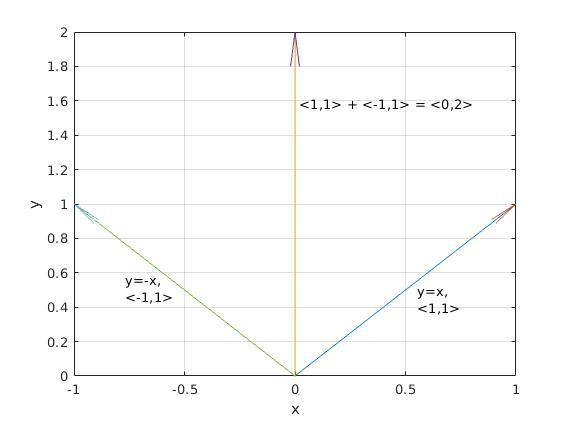
\includegraphics[width=\linewidth]{\resourceDir/img/not_closed_under_addition.png}
	 \caption{The blue arrows are vectors whose scalar multiples will all be in the same line as the blue arrows but the red arrow shows what happens if we add them; the result lies outside of both lines.}
	\end{figure}
	
	
	\paragraph{Is $\R{2}$ a subspace of the complex vector space $\C{2}$?}	
	The definition of a subspace of $\C{2}$ is a set of vectors which is a subset of those in $\C{2}$ and that forms a vector space under the same addition and scalar multiplication of $\C{2}$. The scalar multiplication of the vector space $\C{2}$ is multiplication by scalars $\lambda \in \C{}$.\\
	For a vector, $\v \in \R{2}$, scaling it by a complex number, $\lambda\v$ will result in a vector that is not necessarily in $\R{2}$.
	
	
	\paragraph{Is $\setc{(a,b,c) \in \C{3}}{a^3 = b^3}$ a subspace of $\C{3}$?}
	For $x \in \C{}$, $x^3$ has roots, $1, \frac{-1 + \sqrt{3}i}{2}, \frac{-1 - \sqrt{3}i}{2}$ so we don't have $a = b$ as we would if we were ranging over the reals. \\
	Concretely, we can have, $(1,\frac{-1 + \sqrt{3}i}{2},0)$ and $(1,\frac{-1 - \sqrt{3}i}{2},0)$ but,
	\[ (1,\frac{-1 + \sqrt{3}i}{2},0) + (1,\frac{-1 - \sqrt{3}i}{2},0) = (2,-1,0) \]
	where $(2,-1,0) \not\in \setc{(a,b,c) \in \C{3}}{a^3 = b^3}$ meaning that addition over this set is not closed. Therefore, this is not a subspace.
	
	
	\paragraph{\small{Give an example of a non-empty subset $U$ of $\R{2}$ such that $U$ is closed under addition and under taking additive inverses (meaning $-\u \in U$ whenever $\u \in U$), but $U$ is not a subspace of $\R{2}$.}}
	First thought might be $\R{2} - \{\0\}$ but this is \wrong. If the subset is closed under addition and under taking additive inverses then it means that $\u + -\u = \0 \in U$ and so the set $\R{2} - \{\0\}$ is not closed under addition and taking additive inverses.\\
	The set $\setc{(x,y) \in \R{2}}{x,y \in \Z{}}$ however, is closed under addition because integer addition is closed and under taking additive inverses but scalar multiplication where the scalars range over the reals, will produce non-integer values for $x$ and $y$.

	
	\paragraph{\small{Is the set of periodic functions over the reals a subspace of $\R{R}$?}}{vector problems, periodic functions}{
	The definition of two periodic functions over the reals is
		\begin{align*}		
		\exists p > 0 \in \R{} \cdot f(x) &= f(x + p) \\
		\exists q > 0 \in \R{} \cdot g(x) &= g(x + q) \\
		\end{align*}
	Then for their sum to be periodic we need,
		\begin{align*}
		\exists \alpha, \beta \in \Z{}, m \in \R{} \cdot (m &= \alpha{p}) \wedge (m = \beta{q}) \\[7pt]
		\iff \frac{q}{p} &= \frac{\alpha}{\beta} \in \Q{} \\[7pt]
		\therefore (f + g)(x) = (f + g)(x + m) &= f(x + m) + g(x + m) \\[7pt]
		\iff \frac{q}{p} &\in \Q{}.
		\end{align*}
	}

	\paragraph{\small{Prove that the union of two subspaces of $V$ is a subspace of $V$ if and only if one of the subspaces is contained within the other.}}
		Let $A, B$ be subspaces of $V$ and $\V{a} \in A,\; \V{b} \in B$ and, 
			\[ C = A \cup B = \setc{\V{c}}{\V{c} \in A \;\vee\; \V{c} \in B}. \]
		Since $\V{a},\V{b} \in C$ we have $\text{(C subspace of V)} \iff \forall\alpha,\beta \in F \,\cdot\, (\alpha\V{a} + \beta\V{b}) \in C$. Then,
		\begin{align*}
		\V{b} \in A &\implies \forall\alpha,\beta \in F \,\cdot\, (\alpha\V{a} + \beta\V{b}) \in A \sidecomment{ (by subspace properties) }\\
		&\implies (\alpha\V{a} + \beta\V{b}) \in C.
		\end{align*}
		A similar argument holds for $\V{a} \in B$. Conversely,
		\begin{align*}
		\forall\alpha,\beta \in F \,\cdot\, (\alpha\V{a} + \beta\V{b}) \in C &\implies ((\alpha\V{a} + \beta\V{b}) \in A) \vee ((\alpha\V{a} + \beta\V{b}) \in B)\\
		&\implies ((\alpha\V{a} - \alpha\V{a} + \beta\V{b}) = \beta\V{b} \in A) \vee ((\alpha\V{a} + \beta\V{b} - \beta\V{b}) = \alpha\V{a} \in B)\\
		&\implies (\V{b} \in A) \vee (\V{a} \in B)
		\end{align*}
		\begin{align*}
		\therefore \text{(C subspace of V)} &\iff \forall\alpha,\beta \in F \,\cdot\, (\alpha\V{a} + \beta\V{b}) \in C\\
		&\iff (\V{b} \in A) \vee (\V{a} \in B)\\
		&\equiv (B \subseteq A) \vee (A \subseteq B).
		\end{align*}
	
	
	\paragraph{\small{Can a vector space over an infinite field be a finite union of proper subspaces?}}
		Assume that our vector space V is a finite union of proper subspaces, hence
		\[ V=\bigcup_{i=1}^n U_i. \]
		Now, pick a non-zero vector $ \V{x} \in U_1 $, and pick another vector $ \V{y} \in V\,\backslash U_1. $\\
		
		There are infinitely many vectors $ \V{x} + k\V{y} $, where $ k\in K^* $ ($ K $ is our infinite field). Note that $ \V{x} + k\V{y} $ is not in $ U_1 $, hence must be contained in some $ U_j $ where $ j\neq 1 $.\\
		
		Then since $ k\in K^* $, we can have $ \V{x} + k_1\V{y},\, \V{x} + k_2\V{y} \in U_j $, which implies that it also contains $ \V{y} $ and hence also $ \V{x} $, hence $ U_1\subset U_j $.\\
		
		\textit{Explanation}: There are infinitely many vectors $\V{x} + k\V{y}$ and only finitely many $U_i$ so they cannot all be in different $U_i$ so we have,
		\begin{align*}
		\exists \, k_1,\, k_2 \in K^* \,\cdot\,  \V{x} + k_1\V{y},\, \V{x} + k_2\V{y} \in U_j \\
		\implies (\V{x} + k_1\V{y}) - (\V{x} + k_2\V{y}) = (k_1 - k_2)\V{y} \in U_j \\
		\implies \V{y} \in U_j \implies \V{x} \in U_j
		\end{align*}
		
		Hence
		\[ V=\bigcup_{i=2}^n U_i. \]
		
		Evidently, this can be continued, hence a contradiction arises.\\

	
	\paragraph{\small{Prove or give a counterexample: if $U_1, U_2, W$ are subspaces of $V$ such that $ V = U_1 \oplus W \text{ and } V = U_2 \oplus W $ then $U_1 = U_2$.}}
		Counter example: $V = \F{2}, \; U_1 = \setc{(x, 0) \in \F{2}}{x \in F}, \; U_2 = \setc{(0, x) \in \F{2}}{x \in F}, \; W = \setc{(x, x) \in \F{2}}{x \in F}$.

	
	\bigskip
	\paragraph{\small{Let $U_e$ denote the set of real-valued even functions on $\R{}$ and let $U_o$ denote the set of real-valued odd functions on $\R{}$. Show that $\R{R} = U_e \oplus U_o.$}}
		Every function $f \in \R{R}$ can be expressed as the sum of an even function and an odd function as,
		\[ f(x) = \frac{f(x) + f(-x)}{2} + \frac{f(x) - f(-x)}{2} = g(x) + h(x) \]
	where $g(x) \in U_e$ and $h(x) \in U_o$. So, $U_e + U_o$ spans $\R{R}$.\\
	Furthermore,
	\begin{align*}
	f(x) \in (U_e \cap U_o) &\implies (f(-x) = f(x)) \wedge (f(-x) = -f(x))\\
	&\implies f(x) = -f(x)\\
	&\implies f(x) = 0
	\end{align*}
	Since $f(x) = 0$ is the additive identity of this space, this shows that the intersection is $ \0 $. So, $\R{R} = U_e \oplus U_o.$


	
\pagebreak
\searchableSubsection{Finite Sets of Vectors}{vector spaces}{	
	\bigskip
	
	\subsubsection{Span and Linear Independence}
	\medskip
	\boxeddefinition{
		The \textbf{span} of a nonempty finite set of vectors $S$ -- written ${ span\,S }$ -- is defined as the set of \textbf{finite} linear combinations of elements of $S$,
		\[ \setc{\alpha{_1}\V{v_1} + \alpha{_2}\V{v_2} + \dots + \alpha{_k}\V{v_n}}{\V{v_i} \in S,\, \alpha{_j} \in F}. \]
		The span of an empty set of vectors is defined to be ${ \{\0\} }$.\\\\
		The span of a set $S$ is also sometimes known as the \textbf{subspace generated by $S$}.
	}
	
	\bigskip
	\boxeddefinition{A \textbf{linear relation} among a nonempty finite set of vectors $S$ is any relation of a \textbf{finite} number of elements of $S$ of the form,
		\[ c_1\V{v_1} + \dots + c_n\V{v_n} = \0 \]
		where ${ c_i \in F }$.\\
		A \textbf{linearly independent} set of vectors is a nonempty set among which there is no linear relation except the trivial relation where all ${ c_1, \dots , c_n = 0 }$.\\\\
		The empty set is defined to be linearly independent.
	}

	\note{Note that if we talk about vector spaces being linearly independent this means that their sum is a direct sum. That's to say, if spaces ${ U_1,\dots,U_k }$ are linearly independent and ${ \u_i \in U_i }$ for ${ 1 \leq i \leq k }$, then
		\[ \u_i + \cdots + \u_k = \0 \iff \u_1 = \cdots = \u_k = \0. \]
	}

	\bigskip
	\labeledProposition{If a set of vectors contains the zero vector $\0$ then it cannot be linearly independent.}{set_containing_zero_vector_not_linearly_independent}
	\begin{proof}
		Assume an arbitrary set of vectors ${ \V{v_1}, \dots , \V{v_n} }$ and assume it contains some ${ \V{v_i} = \0 }$. Then we have the linear relation ${ c_i\V{v_i} = \0 }$ with some ${ c_i \neq 0 }$.
	\end{proof}
	\begin{corollary}
		If a set of vectors contains any repitition then it cannot be linearly independent.
	\end{corollary}
	\begin{proof}
		If a set of vectors contains the same vector twice then subtracting one from the other is a non-trivial linear combination of the set of vectors equalling $\0$.
	\end{proof}
	\begin{corollary}
		\label{coro:linearly_independent_iff_vector_reps_are_unique}
		A set of vectors is linearly independent iff, for any vector that may be expressed as a linear combination of vectors in the set, the expression is unique.
	\end{corollary}
	\begin{proof}
		If the expression is not unique then the two different representations may be subtracted one from the other to produce a non-trivial linear combination resulting in $\0$ which contradicts the hypothesis that they are linearly independent. Therefore linearly independent implies unique representation.\\\\
		Conversely, if the set of vectors is not linearly independent then there exists some non-trivial linear combination that results in $\0$. This, in turn, implies that there exists some linear combination of a subset of the vectors that is equal to a linear combination of the remaining vectors. Since these two linear combinations are equal, they represent two different expressions of the same resultant vector. Therefore unique representation implies linearly independent.
	\end{proof}
	
	\bigskip
	\labeledProposition{The span of a list of vectors is the smallest subspace containing those vectors.}{span_smallest_subspace}
	Note that a vector space over $\R{}$ or $\C{}$ is an uncountable set as - while the dimensions of the vector space may be finite - closure under scalar multiplication means that the vectors in the space are continuously valued as the field providing the scalars is continuously valued.\\
	This means that the notion of the \emph{smallest} subspace cannot refer to the cardinality of the set and must refer to ordering based on subset. So, the smallest subspace containing a list of vectors is a subspace that contains the list of vectors and, of which, there is no proper subset which also contains the list of vectors.	
	\begin{proof}
		\begin{align*}
		\text{Let } S &:= span(\V{v_1}, \V{v_2}, \dots , \V{v_k})\\
		 &:= \setc{\alpha{_1}\V{v_1} + \alpha{_2}\V{v_2} + \dots + \alpha{_k}\V{v_k}}{\alpha{_1}, \alpha{_2}, \dots , \alpha{_k} \in F}\\
		\text{and let }V &:= \text{ the smallest vector space containing }\V{v_1}, \V{v_2}, \dots , \V{v_k}.	 
		\end{align*}
		then $S$ contains every linear combination of $\V{v_1}, \V{v_2}, \dots , \V{v_k}$ and nothing else and so is a vector space containing $\V{v_1}, \V{v_2}, \dots , \V{v_k},$\\
		\[ V \subseteq S \]
		Additionally, any vector space containing the vectors $\V{v_1}, \V{v_2}, \dots , \V{v_k}$ must contain all their linear combinations, $span(\V{v_1}, \V{v_2}, \dots , \V{v_k}),$\\
		\[ S \subseteq V \]
		Therefore there is no proper subset of $span(\V{v_1}, \V{v_2}, \dots , \V{v_k})$ that is also a vector space containing $\V{v_1}, \V{v_2}, \dots , \V{v_k},$ and so $span(\V{v_1}, \V{v_2}, \dots , \V{v_k})$ is the smallest vector space containing $\V{v_1}, \V{v_2}, \dots , \V{v_k},$\\
		\[ (V \subseteq S) \wedge (S \subseteq V) \iff V = S \qedhere \]
	\end{proof}

	\bigskip
	\labeledProposition{Let $L$ be a linearly independent set of vectors in $V$ and ${ \v \in V }$. If we add $\v$ to the set $L$ then the resultant set $L'$ is linearly independent iff ${ \v \not\in span\,L }$.}{augmented_linearly_independent_set_lin_ind_iff_added_vec_not_in_span}
	\begin{proof}
		Clearly if ${ \v \in span\,L }$ then the resultant set is linearly dependent.\\
		If ${ v \not\in span\,L }$ however, then if we attempt to form a linear relation of the vectors in $L'$ then we find,
		\[ c_1\V{v_1} + \dots + c_n\V{v_n} + b\v = \0 \]
		implies that ${ b \neq 0 }$ because that would leave a linear relation between the vectors of $L$ which is not possible because $L$ is linearly independent. Therefore,
		\[ \v = -(c_1/b)\V{v_1} + \dots + -(c_n/b)\V{v_n} \]
		which contradicts the assumption that ${ v \not\in span\,L }$.
	\end{proof}
	
	\medskip
	\labeledProposition{If we add a vector ${ \v \in V }$ to a set of vectors $L$ in $V$ to make a new set $L'$, then ${ span\,L = span\,L' }$ iff ${ \v \in span\,L }$.}{augmented_set_of_vectors_has_same_span_if_added_vector_in_span}
	\begin{proof}
		Clearly if ${ \v \in span\,L }$ then adding it to the set $L$ doesn't change its span, so ${ span\,L = span\,L' }$.\\
		Conversely, by construction of $L'$ we have ${ \v \in L' \implies \v \in span\,L' }$ so if ${ span\,L = span\,L' }$ then we also have ${ \v \in span\,L }$.
	\end{proof}
	
	\bigskip
	\labeledProposition{Length of every linearly independent list in a space is less than or equal to the length of a spanning list in the same space.}{independent_list_smaller_than_spanning_list}
	\begin{proof}
	Let $U = \V{u_1}, \V{u_2}, \dots, \V{u_m}$ be a linearly independent list of vectors in $V$ and $W = \V{w_1}, \V{w_2}, \dots, \V{w_n}$ be a spanning list of vectors in $V$.\\
	If we take $\V{u_1}$ from $U$ and add it to $W$ then - since the other vectors in $W$ are a spanning list - $W$ must be linearly dependent. That's to say,
	\begin{align*}
	\exists\,\alpha_1,\alpha_2,\dots,\alpha_n \in \R{} \dotsuchthat &\alpha_1\V{w_1} + \dots + \alpha_n\V{w_n} = \V{u_1} \\[4pt]
	\iff &\alpha_1\V{w_1} + \dots + \alpha_n\V{w_n} - \V{u_1} = -\alpha_i\V{w_i}\\[4pt]
	\iff &\frac{-\alpha_1}{\alpha_i}\V{w_1} + \dots + \frac{-\alpha_n}{\alpha_i}\V{w_n} + \frac{1}{\alpha_i}\V{u_1} = \V{w_i}
	\end{align*}
	So, $\V{w_i}$ is in the span of $\V{u_1}, \V{w_2}, \dots, \V{w_n}$ and we can drop $\V{w_i}$ from the list, $W$, and it will still span the vector space.\\
	We can keep doing this with the remaining vectors in $U$ - each time the vector to be removed will be some $\V{w_i}$ because all the $\V{u_i}$ are linearly independent - and all the while $W$ remains a spanning list. We continue until we have replaced (potentially) all $n$ vectors in $W$, which would happen if $m > n$. At this point we would have the spanning list $W = \V{u_1}, \V{u_2}, \dots, \V{u_n}$ and $(m - n)$ remaining vectors in $U$.\\
	Now, since $W$ spans the space, the $(m - n)$ vectors that remain in $U$ will be in the span of $W$. But, all the vectors that originally came from $U$ were linearly independent, so it is impossible for any vectors in $U$ to be in the span of $W$ (which now comprises only vectors that originally came from $U$).\\
	We therefore conclude that there can be no remaining vectors in $U$ and, consequently that $m$ cannot be greater than $n$, i.e. $m \leq n$.
	\end{proof}

	\bigskip\bigskip
	\note{\textbf{Summary of Span and Linear Independence}\\
		\begin{itemize}
			\item{The span of a set of vectors changes when adding a vector not in the existing span.}
			\item{A linearly independent set of vectors continues to be linearly independent when adding a vector not in the existing span.}
		\end{itemize}
		The fundamental point of linear independence and span is that if the span of two sets of vectors is not completely disjoint (ignoring the zero vector) then the sets are not linearly independent.
		Any nonzero vector in common between the two spans implies a linear relation between the sets,
		\begin{align*}
		&& \V{u_1} + ... + \V{u_n} &= \v = \V{w_1} + ... + \V{w_n} \\
		&\iff & \0 &= (\V{w_1} + ... + \V{w_n}) - (\V{u_1} + ... + \V{u_n}). &\sidecomment{} \\
		\end{align*}
	}


	
	\bigskip
	\subsubsection{Bases}\label{sssection:bases}
	\boxeddefinition{A \textbf{basis} for a vector space $V$ is a set of vectors that is both linearly independent and spans the space $V$. The empty set is therefore a basis for the zero vector space $\{\0\}$.\\
	Since a basis of $V$ spans the space, any vector in $V$ may be expressed as as a linear combination of the vectors in the basis set and, since the basis set is linearly independent, this expression is unique.
	}
	\smallskip\note{Compare with the \textbf{generating set of a group} (\ref{def:generating_set_of_group}).}
	
	\bigskip
	\labeledProposition{A set of vectors ${ B = \{\V{v_1}, \dots , \V{v_n}\} }$ in $V$ is a basis iff every ${ \w \in V }$ can be written in a single unique way as a linear combination of vectors in $B$.}{every_vector_in_space_is_unique_lin_comb_of_basis_vectors}
	\begin{proof}
		If $B$ is a basis of $V$ then, by definition, $B$ spans $V$ and so every ${ \w \in V }$ can be written as a linear combination of vectors in $B$. Furthermore, also by the definition of a basis, the vectors in $B$ are linearly independent so, by corollary \ref{coro:linearly_independent_iff_vector_reps_are_unique} the linear combination is unique.\\\\
		Conversely if every ${ \w \in V }$ can be written in a single unique way as a linear combination of vectors in $B$ then $B$ both spans the space and is linearly independent by corollary \ref{coro:linearly_independent_iff_vector_reps_are_unique}.
	\end{proof}

	\bigskip
	\subsubsection{Examples of Bases}
	\begin{exe}
		\ex{If we take an arbitrary finite set of vectors ${ S = \V{s_1}, \dots, \V{s_n} }$ then the space ${ V = V(S) }$ of linear combinations of elements of $S$ is the set of all expressions of the form,
			\[ a_1\V{s_1}, \dots, a_n\V{s_n}, \hspace{20pt} a_i \in \F{}. \]
			In this space addition and multiplication are carried out assuming no relations among the elements of $S$ so that,
			\[ (a_1\V{s_1} + \dots + a_n\V{s_n}) + (b_1\V{s_1} + \dots + b_n\V{s_n}) = (a_1 + b_1)\V{s_1} + \dots + (a_n + b_n)\V{s_1} \]
			and
			\[ c(a_1\V{s_1} + \dots + a_n\V{s_n}) = ca_1\V{s_1} + \dots + ca_n\V{s_n}. \]
			Then the mapping ${ \phi: \F{n} \longmapsto V(S) }$ defined as,
			\[ \phi(a_1,\dots,a_n) = a_1\V{s_1}, \dots, a_n\V{s_n} \]
			is an isomorphism.
			\note{Note that if the assumption of no relation between the elements of $S$ is not valid then $\phi$ may fail to be isomorphic.}
			$V(S)$ is often referred to as \textit{the space with basis $S$} or \textit{the space of formal linear combinations of $S$}. If $S$ is an infinite set then $V(S)$ is defined to be the set of all \textit{finite} linear combinations of the elements of $S$.\\
			This crops up frequently in applications, when taking weightings of different features for example; this isomorphism allows us to treat them as vectors in $\F{n}$.
		}\label{ex:isomorphism_with_Fn}
	\end{exe}

	

	\bigskip
	\subsubsection{Finite-Dimensional Vector Spaces}
	\boxeddefinition{A vector space is called \textbf{finite-dimensional} if there is some finite set of vectors that spans the space.}
	
	\bigskip
	\labeledProposition{Any finite set which spans a finite-dimensional space contains a basis for the space.}{finite_spanning_set_contains_a_basis}
	\begin{proof}
		Let $S$ be a spanning set of vectors in the space $V$.\\\\
		If $S$ is not linearly independent then there is some ${ \v \in S }$ such that \\${ \v \in span\,(S \setminus \{\v\}) }$. So we can remove $\v$ from the set and $S$ still spans the space. We may continue doing this until $S$ is linearly independent, at which point we have found the minimal subset of $S$ that spans the space. This remaining subset is a basis of the space.
	\end{proof}
	\begin{corollary}
		Any finite-dimensional vector space has a basis.
	\end{corollary}
	\begin{proof}
		This follows from the previous proposition and the definition of a finite-dimensional vector space.
	\end{proof}

	\medskip
	\labeledProposition{Any set (including infinite sets) that spans a finite-dimensional vector space, contains a finite subset which spans the space.}{any_spanning_set_contains_finite_basis}
	\begin{proof}
		Let $V$ be a finite-dimensional vector space and $S$ be a spanning set of $V$. By the definition of $V$ as finite-dimensional there exists some finite set that spans $V$. Let $W$ be a finite set of vectors that spans $V$. Then, since $S$ also spans $V$, every vector in $W$ may be expressed as a finite linear combination of vectors in $S$. The set of all the members of $S$ that participate in the linear combinations required to produce the set $W$ is a finite subset of $S$ that spans $V$.
	\end{proof}
	
	\medskip
	\labeledProposition{Let $V$ be a finite-dimensional vector space. Any linearly independent set ${ L \subseteq V }$ can be extended by adding vectors to obtain a basis of $V$.}{lin_ind_set_can_be_extended_to_basis}
	\begin{proof}
		If $L$ spans $V$ then it is already a basis.\\
		Assume $L$ does not span $V$. Then there exists some ${ \v \in V }$ such that ${ \v \not\in span\,L }$. If we add $\v$ to $L$ then the resulting set, say $L'$, continues to be linearly independent and may or may not span $V$. If it does then $L'$ is a basis. If not then we can continue to repeat the same process until it does span the space at which point we have a basis.
	\end{proof}

	\medskip
	\labeledProposition{For finite subsets of a vector space, any linearly independent set has cardinality less than or equal to that of any spanning set in the same space.}{lin_ind_set_smaller_or_equal_to_a_spanning_set}
	\note{\autoref{prop:lin_ind_set_can_be_extended_to_basis} only tells us that, for any linearly independent set of vectors, there exists some basis whose cardinality is greater than or equal to that of the original set. What we want to prove here is the condition on the cardinality exists between any linearly independent set and spanning set in the same space.}
	\begin{proof}
		We will show two different ways of proving this: one using an algorithm on lists and the other using simultaneous equations.
		\begin{enumerate}[label=(\roman*)]
			\item{\textbf{proof using lists}\\\\
				Let $V$ be a finite-dimensional vector space, $S$ a spanning list ${ \V{s_1}, \dots, \V{s_m} }$ and $L$ a linearly independent list ${ \V{l_1},\dots, \V{l_n} }$ in $V$, and assume that ${ m < n }$.\\
				Now, since $S$ is a spanning list, every element of $L$ is in its span and so if we remove the first element $\V{l_1}$ from $L$ and add it to $S$ then $S$ will definitely contain a linear relation. If we then remove some element $\V{s_i}$ from the original spanning list that participates in a linear relation (i.e. ${ \V{s_i} \in span\,S }$) then we have a modified list $S$, of the same length as the original, but with an element replaced by $\V{l_1}$ and this list continues to span the space.\\
				We can repeat this task $m$ times until all elements $\V{s_i}$ from the original spanning list have been removed and we have a spanning list ${ S = \V{l_1},\dots, \V{l_m} }$ and the remaining ${ n - m }$ elements are still in $L$. But the original ${ L = \V{l_1},\dots, \V{l_n} }$ was linearly independent and no linear relation exists between them so it is impossible that the first $m$ elements span the space because this would mean that they would participate in a linear relation with the remaining ${ n - m }$ elements.\\
				So we have obtained a contradiction and we therefore conclude that ${ m \geq n \qedhere}$.
			}
			\item{\textbf{proof using simultaneous equations}\\\\
				Let $V$ be a vector space, $S$ a finite spanning set ${ \V{s_1}, \dots, \V{s_m} }$ and $L$ a finite linearly independent set ${ \V{l_1},\dots, \V{l_n} }$ in $V$, and assume that ${ m < n }$.\\
				Since $S$ spans the space, every ${ \V{l_j} \in L }$ can be expressed as a linear combination of vectors ${ \V{s_i} \in S }$ of the form,
				\[ \V{l_j} = a_{1j}\V{s_1} + \dots + a_{mj}\V{s_m} = \sum_{i=1}^m a_{ij}\V{s_i} \]
				for ${ 1 \leq j \leq n }$. A linear relation on the vectors of $L$ would look like,
				\begin{align*}
				&& c_1\V{l_1} + \dots + c_n\V{l_n} &= \0 \\
				&\iff & c_1\sum_{i=1}^m a_{i1}\V{s_i} + \dots + c_n\sum_{i=1}^m a_{in}\V{s_i}  &= \0 &\sidecomment{}
				\end{align*}
				which expands into $m$ simultaneous equations as follows.
				\begin{align*}
					c_1a_{11}\V{s_1} + \dots + c_na_{1n}\V{s_1}  &= 0 \\
					. \hspace{100pt} & \\
					. \hspace{100pt} & \\
					c_1a_{m1}\V{s_m} + \dots + c_na_{mn}\V{s_m}  &= 0
				\end{align*}
				As we can see, each of the $m$ equations has a has a factor $\V{s_i}$ in each term and so this may be factored out to give the following system.
				\begin{align*}
					\V{s_1}(c_1a_{11} + \dots + c_na_{1n})  &= 0 \\
					. \hspace{100pt} & \\
					. \hspace{100pt} & \\
					\V{s_m}(c_1a_{m1} + \dots + c_na_{mn})  &= 0
				\end{align*}
				So now we have $m$ equations such that the $i$-th equation will hold if either ${ \V{s_i} = \0 }$ or ${ c_1a_{i1} + \dots + c_na_{in} = 0 }$.\\
				Assume that for all ${ \V{s_i} \in S,\; \V{s_i} \neq \0 }$. Then we end up with the following system.
				\[
					\begin{bmatrix}
					a_{11} & \dots & a_{1n} \\
					. && \\
					. && \\
					a_{m1} & \dots & a_{mn}
					\end{bmatrix}
					\begin{bmatrix}
					c_1 \\
					. \\
					. \\
					c_n
					\end{bmatrix}
					=
					\begin{bmatrix}
					0 \\
					. \\
					. \\
					0
					\end{bmatrix}
				\]
				It can be shown using matrix row reduction that a system such has this has non-trivial solutions if ${ m < n }$. Therefore if ${ m < n }$, there is a linear relation between the vectors of $L$ contradicting its construction as linearly independent. Therefore ${ m \geq n }$.\\\\
				However, there may be some ${ \V{s_i} \in S \suchthat \V{s_i} = \0 }$ but only one because $S$ is a set not a list. If that is all there is (i.e. ${ S = \{\0\} }$) then the space ${ V = \{\0\} }$ and the only linearly independent set of vectors in the zero space is the empty set. In this case ${ n = 0 }$ and so we cannot have ${ m < n }$. Therefore ${ m \geq n }$ also.\\
				On the other hand, if there are non-zero elements in $S$ then we can remove the equation $i$ such that ${ \V{s_i} = \0 }$ so that we will have ${ m - 1 }$ simultaneous equations in our system. But now the linear dependence of $L$ follows if ${ (m-1) < n \iff m < (n+1) }$ and clearly ${ m < n \implies m < n+1 }$ so once again ${ m < n }$ implies that $L$ is not linearly independent. ${ \qedhere }$
			}
		\end{enumerate}
	\end{proof}
	
	\medskip
	\labeledProposition{Any two bases of the same finite-dimensional vector space have the same number of elements. In other words: For a given vector space, the cardinality of bases is fixed.}{basis_cardinality_fixed_for_a_vector_space}
	\begin{proof}
		Let ${ L,L' }$ be finite subsets of the finite-dimensional vector space $V$ such that both are bases. Then both $L$ and $L'$ are linearly independent and span the space. Therefore we have,
		\[ \cardinality{L} \leq \cardinality{L'} \eqand \cardinality{L} \geq \cardinality{L'} \]
		which implies that ${ \cardinality{L} = \cardinality{L'} }$.
	\end{proof}
		
	\medskip
	\subsubsection{Dimension of Finite-Dimensional Vector Spaces}
	\boxeddefinition{The \textbf{dimension} of a finite-dimensional vector space $v$ is the number of vectors in a basis. The dimension will be denoted by ${ dim\,V }$.}
	
	\medskip
	\labeledTheorem{The dimension of a finite-dimensional vector space is an upper bound on the cardinality of a linearly independent set of vectors in the space and a lower bound on the cardinality of a spanning set of vectors in the same space.}{dimension_as_bounds_of_size_of_vector_sets}
	\begin{proof}
		This theorem follows from \autoref{prop:lin_ind_set_smaller_or_equal_to_a_spanning_set}.
	\end{proof}

	\medskip
	\labeledTheorem{Any linearly independent set of vectors in a finite-dimensional vector space $V$ of cardinality ${ dim\,V }$ is a basis.}{lin_ind_set_of_dim_cardinality_is_basis}
	\begin{proof}
		Let ${ L \subset V }$ be linearly independent set of vectors in $V$ with ${ \cardinality{L} = dim\,V }$. By \autoref{prop:lin_ind_set_can_be_extended_to_basis}, any linearly independent set in $V$ may be extended with zero or more vectors to obtain a basis ov $V$. But any basis of $V$ has dimension ${ dim\,V = \cardinality{L} }$. Therefore we extend $L$ with zero vectors to obtain a basis.
	\end{proof}


	\medskip
	\labeledProposition{If ${ W \subseteq V }$ is a subspace of a finite-dimensional vector space then,
		\[ dim\,W \leq dim\,V \eqand (dim\,W = dim\,V) \iff (W = V). \]
	}{subspace_dimension_leq_dimension_of_parent_space}
	\begin{proof}
		Firstly note that $W$ must also be finite-dimensional because by definition there is a finite set of vectors that spans $V$ and since ${ W \subseteq V }$, the same set must also span $W$.\\
		Every basis of $W$ is also a linearly independent set in $V$ and so, by \autoref{prop:lin_ind_set_smaller_or_equal_to_a_spanning_set}, it cannot have cardinality greater than any basis of $V$. Any basis in $V$ has cardinality ${ dim\,V }$ so the cardinality of any basis of $W$ must be less than or equal to ${ dim\,V }$. Therefore ${ dim\,W \leq dim\,V }$.\\
		
		If ${ dim\,W = dim\,V }$ on the other hand, every basis of $W$ has the same cardinality as every basis of $V$. Since every basis of $W$ is also a linearly independent set in $V$ with cardinality equal to ${ dim\,V }$, by \autoref{theo:lin_ind_set_of_dim_cardinality_is_basis} it is a basis of $V$. By similar logic in reverse, any basis of $V$ is also a basis of $W$.\\
		Let $B$ be such a basis. Then,
		\[ \v \in W \iff \v \in span\,B \iff \v \in V. \]
		Therefore ${ W = V }$.
	\end{proof}

	\medskip
	\labeledTheorem{Let ${ W_1, W_2 }$ be subspaces of a finite-dimensional vector space. Then,
		\[ dim(W_1 + W_2) = dim\,W_1 + dim\,W_2 - dim(W_1 \cap W_2). \]
	}{dimension_follows_set_cardinality_law}
	\begin{proof}
		It is easy to show that the intersection of two subspaces is a subspace. So define a basis of ${ W_1 \cap W_2 }$ as ${ B = \{\V{u_1}, \dots, \V{u_r}\} }$ where ${ r = dim(W_1 \cap W_2) }$.\\
		Then $B$ is a linearly independent set in $W_1$ and can be extended to a basis of $W_1$,
		\[ B_{W_1} = \{\V{u_1}, \dots, \V{u_r}, \V{v_1}, \dots, \V{v_{m-r}}\} \]
		where ${ m = dim\,W_1 }$.\\
		By the same reasoning we can extend $B$ to a basis of $W_2$,
		\[ B_{W_2} = \{\V{u_1}, \dots, \V{u_r}, \V{w_1}, \dots, \V{w_{n-r}}\} \]
		where ${ n = dim\,W_2 }$.\\
		Now if we can show that,
		\[ B' = B_{W_1} \cup B_{W_2} = \{ \V{u_1}, \dots, \V{u_r}, \V{v_1}, \dots, \V{v_{m-r}}, \V{w_1}, \dots, \V{w_{n-r}} \} \]
		is a basis of ${ W_1 + W_2 }$ then the proof will follow easily.\\
		Clearly, $B'$ spans ${ W_1 + W_2 }$ as $B'$ contains a basis of both $W_1$ and $W_2$ and so is able to express any sum of two vectors chosen from the two spaces.\\
		Linear Independence is a little more complicated however. Consider that, since $B_{W_1}$ is linearly independent, there can be no linear relation between the vectors $\V{u_i}$ and $\V{v_i}$ and similarly there can be no such relation between the vectors $\V{u_i}$ and $\V{w_i}$. Therefore, if there were to be a linear relation among the vectors it would have to involve the vectors $\V{v_i}$ with the vectors from $B_{W_2}$ or the vectors $\V{w_i}$ with the vectors from $B_{W_1}$. If we model the linear relation as a relation between vectors that are linear combinations of the vectors $\V{u_i}, \V{v_i}$ and $\V{w_i}$ we get,
		\[ \u + \v + \w = \0 \iff \v = -\u - \w \in W_2 \]
		therefore ${ \v \in W_1 \cap W_2 }$ and so $\v$ can be expressed as a linear combination of the vectors in $B$. But this implies a linear relation among the vectors of $B_{W_1}$ which are linearly independent by construction. Therefore 
		\[ \v = \0 \implies -\u - \w = \0 \iff -\u = \w \]
		which implies that there is a linear relation among the vectors of $B_{W_2}$ which are also linearly independent by construction and so ${ \u = \w = \0 }$.
	\end{proof}
	\begin{corollary}
		\label{coro:dimension_of_set_of_subspaces_leq_sum_of_dimension_of_each_subspace}
		Let ${ W_1, \dots, W_n }$ be a set of subspaces of a finite-dimensional vector space. Then,
		\[ dim(W_1 + \cdots + W_n) \leq dim\,W_1 + \cdots + dim\,W_n \]
		with the equality case iff the spaces ${ W_1, \dots, W_2 }$ are independent.
	\end{corollary}
	\begin{proof}
		This follows by induction on \autoref{theo:dimension_follows_set_cardinality_law}.\\		
		If we take the case of ${ n = 2 }$ as our base case then,
		\[ dim(W_1 + W_2) = dim\,W_1 + dim\,W_2 - dim(W_1 \cap W_2) \leq dim\,W_1 + dim\,W_2. \]
		Furthermore, if ${ W_1, W_2 }$ are independent then ${ W_1 \cap W_2 = \{\0\} }$ so that,
		\[ dim(W_1 + W_2) = dim\,W_1 + dim\,W_2 - 0 = dim\,W_1 + dim\,W_2. \]
		For the induction step: Let ${ W' = W_1 + \cdots + W_{n-1} }$ and take as the induction hypothesis that,
		\[ dim(W') \leq dim\,W_1 + \cdots + dim\,W_{n-1} \]
		with equality being when the spaces are independent. Then observe that, by the associativity of addition of vectors and hence of vector spaces,
		\begin{align*}
		&& dim(W_1 + \cdots + W_n) &= dim((W_1 + \cdots + W_{n-1}) + W_n)  \\
		& &  &= dim\,W' + dim\,W_n - dim(W' \cap W_n)  &\sidecomment{by \autoref{theo:dimension_follows_set_cardinality_law}} \\
		& &  &\leq dim\,W' + dim\,W_n \\
		& &  &\leq dim\,W_1 + \cdots + dim\,W_{n-1} + dim\,W_n  &\sidecomment{by induction hypothesis.}
		\end{align*}
		Furthermore, if ${ dim\,W' = dim\,W_1 + \cdots + dim\,W_{n-1} }$ and if the spaces $W'$ and $W_n$ are independent then the intersection,
		\[ W' \cap W_n = \{\0\} \]
		which gives,
		\begin{align*}
		&& dim(W_1 + \cdots + W_n) &= dim((W_1 + \cdots + W_{n-1}) + W_n)  \\
		& &  &= dim\,W' + dim\,W_n - 0  &\sidecomment{by \autoref{theo:dimension_follows_set_cardinality_law}} \\
		& &  &= dim\,W_1 + \cdots + dim\,W_{n-1} + dim\,W_n  &\sidecomment{by induction hypothesis.}
		\end{align*}
		This shows that if the spaces are independent then 
		\[ dim(W_1 + \cdots + W_n) = dim\,W_1 + \cdots + dim\,W_n \]
		but it is also easy to reverse the logic and show that if the above equality holds then, if we add a space to the sum of other spaces, then the intersection of the added space with the sum of the other spaces must have dimension 0 and therefore must be $\{\0\}$. In this way we can also prove the converse implication that the spaces must be independent.
	\end{proof}

	\bigskip
	\labeledProposition{Two finite-dimensional vector spaces may be isomorphic only if they have the same dimension.}{isomorphism_between_two_vector_spaces_implies_same_dimension}
	\begin{proof}
		We want to prove that if ${ \phi: W \longmapsto V }$ is an isomorphism of vector spaces then it follows that ${ dim\,W = dim\,V }$.\\
		Assume for contradiction that $\phi$ is indeed an isomorphism between the vector spaces $W$ and $V$ but,
		\[ dim\,W = m > dim\,V = n. \]
		Then any basis of ${ \V{w_1}, \dots, \V{w_m} \in W }$ is a linearly independent set of vectors in $W$ with the property, for ${ c_1,\dots,c_m \in \F{} }$,
		\begin{align*}
		&& c_1\V{w_1} + \dots + c_m\V{w_m} &= \0 \iff c_1,\dots,c_m = 0  \\
		&\iff & \phi(c_1\V{w_1} + \dots + c_m\V{w_m}) &= \phi(\0) = \0 \iff c_1,\dots,c_m = 0 \\
		&\iff & c_1\phi(\V{w_1}) + \dots + c_m\phi(\V{w_m}) &= \0 \iff c_1,\dots,c_m = 0. \\
		\end{align*}
		But we have ${ \phi(\V{w_1}), \dots, \phi(\V{w_m}) \in V }$ so that the result obtained implies that ${ \phi(\V{w_1}), \dots, \phi(\V{w_m}) }$ is a linearly independent set of vectors in $V$ of cardinality ${ m > n = dim\,V }$. By \autoref{theo:dimension_as_bounds_of_size_of_vector_sets} this cannot be and we have obtained a contradiction. 
	\end{proof}

	\bigskip
	\TODO{example application of calculating the order of $GL_2(\F{})$ when ${ \F{} = \F{}_p }$ is a prime field. Artin[114]}	
	
	\bigskip
	\subsubsection{Direct Sums in Finite-Dimensional Vector Spaces}
	\medskip
	\labeledProposition{Let ${ W_1, \dots, W_n }$ be subspaces of a finite-dimensional vector space $V$, and let $B_i$ be a basis for $W_i$. Then, the union
		\[ \bigcup_{i=1}^n B_i \]
		is a disjoint union and forms a basis of $V$ iff 
		\[ V = W_1 \otimes \cdots \otimes W_n. \]
	}{bases-of-direct-summands-have-disjoint-union-equal-to-basis-of-space}
	\begin{proof}
		Let ${ B = \bigcup_i B_i }$ be a basis of $V$. Then $B$ is a linearly independent set and so,
		\[ \forall \V{b} \in B \logicsep \V{b} \not\in span(B \setminus \{\V{b}\}) \]
		which also means that,
		\[ \forall B_i \subset B \logicsep span\,B_i \cap span(B \setminus B_i) = \0. \]
		This implies that the sets $B_i$ are independent spaces. Since their union is a basis of $V$ then together they span $V$. Since the span of each $B_i$ is $W_i$ then, ${ V = W_1 \oplus \cdots \oplus W_n }$.\\
		Conversely, if ${ V = W_1 \oplus \cdots \oplus W_n }$ then each subspace $W_i$ is independent so that, for every ${ \V{b} \in B_i,\; \V{b} \not\in span(B \setminus B_i) }$. This means that if we begin with $B_1$ and add to it the elements of $B_2$ then the resulting set remains linearly independent and we can continue this until we have ${ B = \bigcup_i B_i }$ as a linearly independent set. Then $B$ contains all the basis vectors of every $W_i$ and therefore, by ${ V = W_1 \oplus \cdots \oplus W_n }$, $B$ spans the space $V$. It is therefore a basis of $V$.
	\end{proof}

	\medskip
	\labeledProposition{Let $W$ be a subspace of a finite-dimensional vector space $V$. Then there is another subspace $W'$ such that ${ W \oplus W' = V }$.}{subspaces-have-a-complement-wrt-direct-sum}
	\begin{proof}
		Any basis of $W$ is a linearly independent set in $V$ and can be extended to a basis of $V$ by adding a set of linearly independent vectors $S$. Then $S$ is a basis of a subspace $W'$ such that any vector in $V$ is in ${ W + W' }$ and since their bases are linearly independent this sum of spaces is a direct sum ${ W \oplus W' }$. Therefore, ${ W \oplus W' = V }$.
	\end{proof}
	\note{Notes about \autoref{prop:subspaces-have-a-complement-wrt-direct-sum}:
		\begin{itemize}
			\item{It is not necessary that there be only one such subspace $W'$. In fact, often there are an infinite number of such subspaces. All such spaces are isomorphic.}
			\item{The proposition that all subspaces have a complement space can also be proven for infinite-dimensional spaces if we use the Axiom of Choice (\ref{sssection:axiom-of-choice}).}
		\end{itemize}
	}
	
	\bigskip
	\subsubsection{Vector Complement Spaces and Quotient Spaces}
	\boxeddefinition{\textbf{(Complement Space)} A subspace $W'$ of a finite-dimensional vector space $V$ such that ${ W \oplus W' = V }$ is called a \textit{complement space}. While there may be many such spaces $W'$, they are equivalent upto isomorphism.
	}\label{def:vector-complement-space}
	\boxeddefinition{The subspace $W'$ of $V$ such that ${ W \oplus W' = V }$ is called the \textbf{quotient space of $V$ by $W$} and is denoted ${ V/W }$. \wrong 
		\TODO{copy correct definition from wikipedia}
	}\label{def:vector-quotient-space}
	
	Further information: \href{https://en.wikipedia.org/wiki/Quotient_space_(linear_algebra)}{wikipedia}.
	
	\biggerskip
	\begin{exe}
		\ex{Consider the vector space $\R{2}$ and let $W$ be the subspace created by the linear combinations of the vector ${ (1,1)^T }$ --- i.e. the line ${ y = x }$ shown in red in the diagrams below.\\
			
		\begin{figure}[h!]
			\centering
			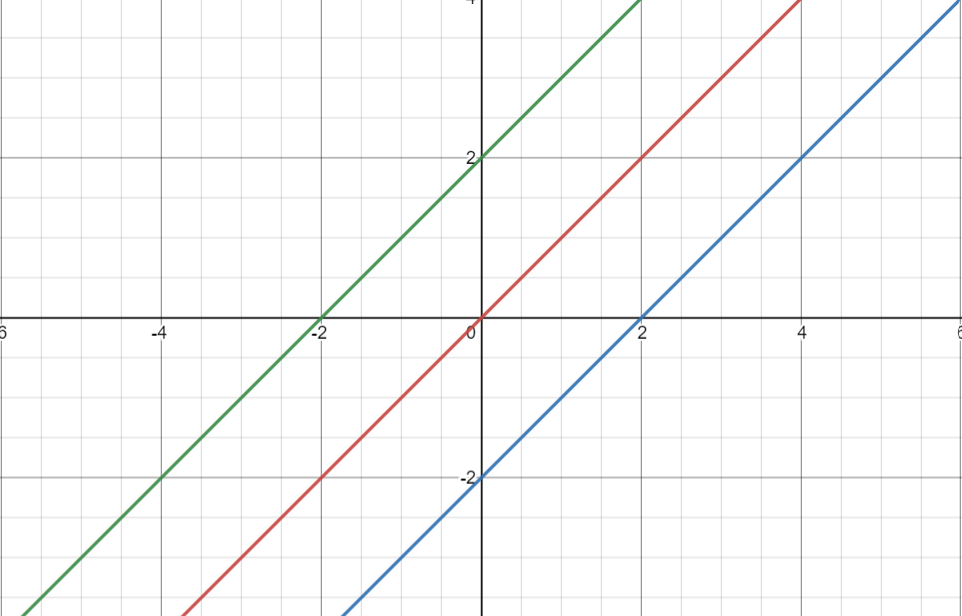
\includegraphics[width=200pt]{\resourceDir/img/vector_cosets_in_quotient_space.png}
			\caption{The green and blue lines are both cosets of $W$ in $\R{2}$ and elements in the quotient space.}
			\label{fig:vector_cosets_in_quotient_space}
		\end{figure}
	
		\autoref{fig:vector_cosets_in_quotient_space} shows two of the cosets of $W$ in $\R{2}$ as green and blue lines. The cosets such as these are the elements of the quotient space and they are the infinite number of lines parallel to ${ y = x }$. They are parallel because they are affine spaces whose associated vector space is the linear combinations of ${ (1,1)^T }$ --- these linear combinations form the kernel of the quotient map and the elements of the quotient space are the additive cosets with the kernel of the quotient map.\\
		
		\autoref{fig:vector_subspaces_isomorphic_to_quotient_space} shows two of the complement spaces as green and blue lines. Such complement spaces are the subspaces $W'$ of $\R{2}$ such that ${ W \oplus W' = \R{2} }$. Any non-parallel line is such a subspace. Each point on such a line represents a vector that is an element of the complement space and is also a point in a line parallel to ${ y = x }$. In this way, any one of the possible complement spaces $W'$ is isomorphic to the quotient space.
		
		\begin{figure}[h!]
			\centering
			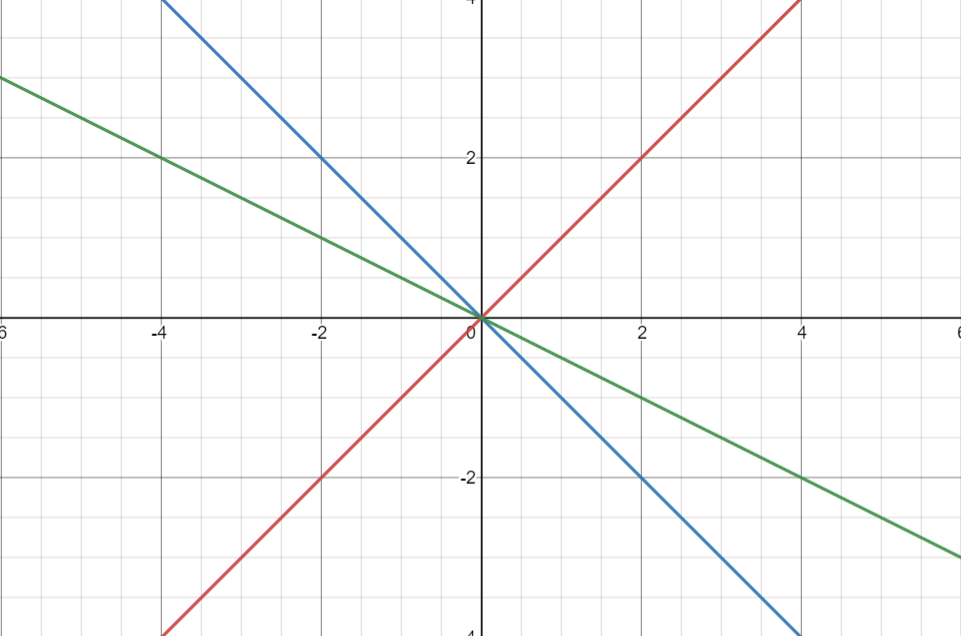
\includegraphics[width=200pt]{\resourceDir/img/vector_subspaces_isomorphic_to_quotient_space.png}
			\caption{The green and blue lines are both complement spaces --- subspaces $W'$ such that ${ W \oplus W' = \R{2} }$.}
			\label{fig:vector_subspaces_isomorphic_to_quotient_space}
		\end{figure}	
		}
	\end{exe}
	\clearpage
	
}




% ----------------


\pagebreak
\searchableSubsection{Infinite Sets of Vectors}{vector spaces, analysis}{	
	
	\bigskip
	The definition of a vector space defines what it means to add two vectors and so, by extension, arbitrarily large \textit{finite} sums of vectors but not what it means to add an infinite number of vectors. Therefore, we define the span and linear independence of infinite sets of vectors as conditions over finite subsets of the vectors.
	
	\bigskip
	\subsubsection{Span and Linear Independence of Infinite Sets of Vectors}
	\boxeddefinition{The \textbf{span of an infinite set of vectors} $S$ is defined to be the set of \textbf{finite} linear combinations of its elements,
		\[ \setc{ c_1\V{v_1} + \dots + c_r\V{v_r} }{ \V{v_i} \in S,\, c_i \in \F{} } \]
		where $r$ is finite but may be arbitrarily large.
	}
	\medskip
	\boxeddefinition{An \textbf{infinite set of vectors} is defined to be \textbf{linearly independent} if there is no linear relation among a \textbf{finite} subset of them,
		\[ c_1\V{v_1} + \dots + c_n\V{v_n} = \0 \]
		where ${ c_i \in F }$.\\
	}

	\note{These definitions of span and linear independence are compatible with the corresponding definitions for finite sets of vectors.}
	
	\bigskip
	\subsubsection{Infinite-Dimensional Vector Spaces}
	\boxeddefinition{A vector space is called \textbf{infinite-dimensional} if there is no finite set of vectors that spans the space.}
	
	
	\bigskip
	\subsubsection{Examples of Infinite-Dimensional Vector Spaces}
	\begin{exe}
		\ex{The space $\R{\infty}$ of infinite real vectors ${ (a) = (a_1,a_2,a_3,\dots) }$ can also be thought of as the space of sequences $\{a_n\}$ of real numbers. It has many important subspaces:
			\begin{xlist}
				\ex{Convergent sequences: ${ C = \setc{(a) \in \R{\infty}}{\lim_{n \to \infty} a_n \text{ exists}} }$.}
				\ex{Bounded sequences: ${ l^{\infty} = \setc{(a) \in \R{\infty}}{\{a_n\} \text{ is bounded}} }$.}
				\ex{Absolutely convergent series: ${ l^1 = \setc{(a) \in \R{\infty}}{\sum_1^{\infty} \abs{a_n} < \infty} }$.}
				\ex{Sequences with finitely many nonzero terms: 
					\[ Z = \setc{(a) \in \R{\infty}}{a_n = 0 \text{ for all but finitely many }n}. \]
				}\label{ex:vec_space_finite_sequences}
			\end{xlist}
		}
	\end{exe}

	\bigskip
	\subsubsection{Bases of Infinite-Dimensional Vector Spaces}
	\boxeddefinition{As with finite sets, a \textbf{basis of an infinite-dimensional vector space} is a linearly independent set which spans the space.}
	
	\bigskip
	\begin{exe}
		\item{Let ${ S = (e_1,e_2,\dots) }$ be the infinite set of standard basis vectors in $\R{\infty}$. $S$ does not span $\R{\infty}$ because the vector ${ \V{w} = (1,1,1,\dots) }$ is not a \textit{finite} linear combination of the elements of $S$. It \textit{is}, however, a basis of the vector space $Z$ in \ref{ex:vec_space_finite_sequences}.
		}
	\end{exe}

	\note{It can be shown, using the Axiom of Choice, that every vector space has a basis (\autoref{theo:every-vector-space-has-basis}) but a basis of $\R{\infty}$ will be uncountably infinite and so will not be expressable as ${ (\V{v_1},\V{v_2},\dots) }$.}
	
	From \href{http://www.math.lsa.umich.edu/~kesmith/infinite.pdf}{the University of Michigan Maths Dept. Linear Algebra Supplement on Infinite-Dimensional Vector Spaces}:
	\note{Let $\R{}$ be the set of real numbers considered as a vector space over the field $\Q{}$ of rational numbers. What could possibly be a basis? The elements $\sqrt{2}, \sqrt{3}, \sqrt{5}, \sqrt{6}, \dots$ can be shown to be linearly independent, but they certainly don’t span $\R{}$, as we also need elements like $\pi, \pi^2, \pi^3, \dots$, which also form a linearly independent set. In fact, because $\Q{}$ is countable, one can show that the subspace of $\R{}$ generated by any countable subset of $\R{}$ must be countable. Because $\R{}$ itself is uncountable, no countable set can be a basis for $\R{}$ over $\Q{}$. This means that any
	basis for $\R{}$ over $\Q{}$, if one exists, is going to be difficult to describe.}
	
	If we were to look for a basis of the functions over the reals we could consider the indicator functions for all ${ r \in \R{} }$,
	\[ i_r(x) \coloneqq 
	\begin{cases}
		1 & x = r\\
		0 & x \neq r
	\end{cases}. 
	\]
	This set of functions is clearly linearly independent and spans the set of functions ${ \R{} \longmapsto \R{} }$. Since there is one such indicator function for each real number and the real numbers are uncountable, this set of indicator functions is also uncountable.
	
	\labeledTheorem{A linear operator over an infinite-dimensional vector space does not conform to the Dimension Formula for finite-dimensional vector spaces.}{no-dimension-formula-for-infinite-vector-spaces}
	\begin{proof}
		The shift operator described in a note to \autoref{prop:properties_of_non_bijective_lin_operator}) is an example of a linear transformation over an infinite-dimensional vector space that doesn't conform to the dimension formula. As noted there, the reason is that infinite sets may have proper subsets of equal cardinality. So we can have an image that is clearly "smaller" than the space but nevertheless has the same dimensionality and so the map has a trivial kernel anyway.\\
		Conversely the differentiation operator has a non-trivial kernel (the set of constant polynomials) but when differentiating an infinite power series the result is still an infinite power series.
	\end{proof}

	\bigskip\note{There is much more to this topic. For more details see \href{http://www.math.lsa.umich.edu/~kesmith/infinite.pdf}{the University of Michigan Maths Dept. Linear Algebra Supplement on Infinite-Dimensional Vector Spaces}.}
}



% -----------------



\pagebreak
\searchableSubsection{Coordinate Vector Spaces}{vector spaces}{
	\bigskip
	\boxeddefinition{A \textbf{coordinate vector} is a representation of a vector as an ordered list of numbers that describes the vector in terms of a particular ordered basis.}
	
	\medskip\boxeddefinition{Let ${ B = \{\v_1, \dots, \v_n\} }$ be a basis of a finite-dimensional vector space $V$. Then for every ${ \v \in V }$ it is possible to express $\v$ as a linear combination of the vectors in $B$ in the form,
		\[ \v = c_1\v_1 + \cdots + c_n\v_n. \]
		Then, the \textbf{coordinate vector of $\v$ with respect to the basis $B$} is,
		\[ \v_B = \langle c_1, \dots, c_n \rangle. \]
	}

	\medskip\note{The definition of a basis \ref{sssection:bases} requires that it is a set of \textbf{linearly independent} vectors. It is worth noting what results if we attempt to use a linearly dependent set of vectors as a basis because in real-world situations this often occurs (for example in data analysis) when the full relationship between objects may not be known.\\
	Imagine a "basis" ${ B = \{x, 3x\}. }$ Co-ordinate vectors defined against this basis are not unique --- 
		\[ (3)x + (1)3x = (6)x + (0)3x = \cdots \]
	In fact, from the basis and the co-ordinate vectors, we appear to working in a 2-dimensional space but in fact, because there is a linear relation between the two "basis" vectors we are actually working in a 1-dimensional space. As a result, algebraic analysis will be missing one relation. For example, take the vectors against "basis" $B$,
	\[ \left\{ \begin{bmatrix}1\\0\end{bmatrix}, \begin{bmatrix}1\\3\end{bmatrix}, \begin{bmatrix}1\\5\end{bmatrix} \right\}. \]
	It appears that there is a single linear relation between these vectors given by the nullspace of their matrix as follows:
	\[ 	\begin{bmatrix}
			1 & 1 & 1\\
			0 & 3 & 5
		\end{bmatrix} \leadsto
		\begin{bmatrix}
			1 & 0 & -2/3\\
			0 & 1 & 5/3
		\end{bmatrix} \implies
		\text{nullspace} =
		t\begin{bmatrix}
			2/3\\
			-5/3\\
			1
		\end{bmatrix} \hspace{20pt} \text{ for } t \in \R{}.
	\]
	Whereas in actual fact all vectors in this space are colinear, being of the form ${ \alpha x }$ for some ${ \alpha \in \R{} }$. If we apply the co-ordinate vectors to their "basis" we see that,
	\[ \begin{bmatrix}1\\0\end{bmatrix} = (1)x = \bm{x}, \begin{bmatrix}1\\3\end{bmatrix} = (1)x + (3)3x = \bm{10x}, \begin{bmatrix}1\\5\end{bmatrix} = (1)x + (5)3x = \bm{16x}. \]
	Then we can see that the true extent of the relationship between the vectors is given by,
	\[ \begin{bmatrix}1 & 10 & 16\end{bmatrix} \leadsto s \begin{bmatrix}-10\\1\\0\end{bmatrix} + t \begin{bmatrix}-16\\0\\1\end{bmatrix} \]
	for ${ s,t \in \R{} }$.\\
	As we can see, the true relation (with respect to $x$) between the vectors is 2-dimensional. The relation found when using the "basis" $B$ is a 1-dimensional subspace within this space corresponding to the values ${ s = -5/3,\; t = 1 }$.
	}
	
	\biggerskip
	\boxeddefinition{The \textbf{dot product} of two coordinate vectors in an $n$-dimensional coordinate space is defined as,
		\[ \v \dotprod \w = v_1w_1 + \cdots + v_nw_n = \v^T\w. \]
	}\label{defn:dot-product}

	\notation{The \textbf{dot product} may also be denoted ${ \langle \v,\w \rangle }$ but this notation may also refer to a literal coordinate vector, i.e.
		\[ \begin{bmatrix}3\\7\end{bmatrix} = \langle 3,7\rangle = (3,7)^T. \]
	}

	\bigskip
	\labeledProposition{The properties of the dot product are:
		\newcommand\vx{\V{x}}
		\newcommand\vy{\V{y}}
		\newcommand\vz{\V{z}}
		\begin{enumerate}[label=(\roman*)]
			\item{$\langle \vx, \vy \rangle = \langle \vy, \vx \rangle$}
			\item{$\alpha\langle \vx, \vy \rangle = \langle \alpha \vx, \vy \rangle = \langle \vx, \alpha \vy \rangle$}
			\item{$\langle \vx+\vy, \vz \rangle = \langle \vx, \vz \rangle + \langle \vy, \vz \rangle$}
			\item{$\langle \vx, \vx \rangle \geq 0$ and $\langle \vx, \vx \rangle = 0 \iff \vx = 0$}
		\end{enumerate}
	}{properties_of_dot_product}
	\begin{proof}
		\newcommand\vx{\V{x}}
		\newcommand\vy{\V{y}}
		\newcommand\vz{\V{z}}
		Proofs of these properties follow from the definition of the dot product.
		\begin{enumerate}[label=(\roman*)]
			\item{$\langle \vx, \vy \rangle = \langle \vy, \vx \rangle$ follows from the commutativity of multiplication in a field,
				\[ x_iy_i = y_ix_i. \]
			}
			\item{$\alpha\langle \vx, \vy \rangle = \langle \alpha \vx, \vy \rangle = \langle \vx, \alpha \vy \rangle$ follows from the associativity of multiplication in a field, 
				\[ \alpha x_i y_i = x_i \alpha y_i. \]
			}
			\item{$\langle \vx+\vy, \vz \rangle = \langle \vx, \vz \rangle + \langle \vy, \vz \rangle$ follows from the distributivity of multiplication over addition in a field,
				\[ (x_i + y_i)z_i = x_iz_i + y_iz_i. \]
			}
			\item{$\langle \vx, \vx \rangle \geq 0$ and $\langle \vx, \vx \rangle = 0 \iff \vx = 0$ follows from its form as a sum of squares,
				\[ x_1^2 + x_2^2 + \cdots + x_n^2. \]
			}
		\end{enumerate}
	\end{proof}
	
	\bigskip
	\subsubsection{Examples of coordinate vectors}
	\begin{exe}
		\ex{Let ${ \x = \langle 3, 3 \rangle \in \R{2} }$ and $B$ be the set ${ \{\langle 2, 0 \rangle, \langle 1, 3 \rangle\} }$ so that $B$ is a non-standard basis of the space $\R{2}$. Then we can also define $\x$ with respect to the basis $B$ as follows.
			\[ \x =
			1\cdot\begin{bmatrix}
			2\\
			0
			\end{bmatrix} +
			1\cdot\begin{bmatrix}
			1\\
			3
			\end{bmatrix}
			\]
			Therefore, the \textbf{coordinate vector of $\x$ with respect to the basis $B$} is defined as,
			\[ \x_B = \langle 1, 1 \rangle. \]
		}
	\end{exe}
	

	\medskip
	\subsubsection{Bases as Matrices}
	\medskip
	\notation{If ${ B = \{\v_1, \dots, \v_n\} }$ is a set of vectors then, when it seems necessary to clearly differentiate, the matrix whose columns are the elements of $B$ will be denoted $[B]$. However, for convenience, when the mathematical context makes clear whether we are referring to a set of vectors or a matrix we will use $B$ to indicate either the set or the matrix.
	}
	
	\medskip
	\labeledProposition{If $\x_B$ is a coordinate vector of $\x$ \wrt the basis $B$ then left multiplication by the matrix $[B]$ whose columns are the elements of $B$ converts $\x_B$ to its standard coordinate form $\x$,
		\[ \x = [B]\x_B. \]
	}{left_multipy_coords_by_basis_gives_standard_coords}
	\begin{proof}
		Let ${ B = \{\v_1, \dots, \v_n\} }$ be a basis and the basis matrix
		\[ [B] = \begin{bmatrix} \v_1 & \dots & \v_n \end{bmatrix} \]
		and ${ \x = \langle x_1,\dots,x_n \rangle }$ is a vector in standard coordinates.
		Then if we calculate $\x$ using the basis $B$,
		\[ \x = x_{B1}\v_1 + \cdots + x_{Bn}\v_n \]
		we get a coordinate vector \wrt $B$,
		\[ \x_B = \langle x_{B1}, \dots, x_{Bn} \rangle. \]
		So, clearly, to recover the standard coordinate vector we need to apply $\x_B$ to the basis against which it was defined,
		\[ [B]\x_B = \begin{bmatrix} \v_1 & \dots & \v_n \end{bmatrix}
					 \begin{bmatrix}  x_{B1} \\ \vdots \\ x_{Bn} \end{bmatrix} =
					 x_{B1}\v_1 + \cdots + x_{Bn}\v_n = \x.  \qedhere
		\]
	\end{proof}
	\begin{corollary}
		If $\x$ is a coordinate vector \wrt the standard basis and $B$ is an alternative basis then left multiplication by the matrix $\inv{[B]}$ converts $\x$ to $\x_B$ its form \wrt the basis $B$.
	\end{corollary}
	\begin{proof}
		\[ [B]\x_B = \x \iff \x_B = \inv{[B]}\x. \]
	\end{proof}

	\medskip
	\note{One way to think of the action of the basis matrix is that it is used to encode/decode coordinates into/from its basis coordinates.\\
		For example, if $\x_B$ is a coordinate vector \wrt the basis $B$, then left-multiplying it by the basis matrix $[B]$,
		\[ \x = [B]\x_B \]
		decodes the coordinate vector into standard coordinates. Conversely we can use the inverse of the basis matrix,
		\[ \x_B = \inv{[B]}\x \]
		to encode a standard coordinate vector into $B$-coordinates.
	}
	
	\bigskip
	\subsubsection{Relationship with Abstract Vector Spaces}
	\medskip
	\labeledProposition{Every vector space $V$ of dimension $n$ is isomorphic to the space $\F{n}$ of column vectors.}{vector_space_isomorphic_to_coordinate_space_of_same_dimension}
	\begin{proof}
		Let ${ \phi: \F{n} \longmapsto V }$ be defined as ${ \phi(\V{x}) = B\V{x} }$ where $B$ is a matrix whose columns are a basis of $V$. The map $\phi$ is surjective because the columns of $B$ span the space $V$ and it is injective because they are linearly independent. So $\phi$ is a bijection.\\
		The structure of the vector space is preserved because,
		\[ \phi(\V{x_1} + \V{x_2}) = B(\V{x_1} + \V{x_2}) = B\V{x_1} + B\V{x_2} = \phi(\V{x_1}) + \phi(\V{x_2}) \]
		and
		\[ \phi(c\V{x}) = B(c\V{x}) = cB\V{x} = c\phi(\V{x}). \]
	\end{proof}

	\medskip
	\note{Note that, by \autoref{prop:isomorphism_between_two_vector_spaces_implies_same_dimension}, $\F{n}$ is \textbf{not} isomorphic to $\F{m}$ for ${ m \neq n }$. Every finite-dimensional vector space $V$ is isomorphic to $\F{n}$, for some uniquely determined integer $n$.\\
		So, the finite-dimensional vector spaces are completely classified by \autoref{prop:vector_space_isomorphic_to_coordinate_space_of_same_dimension} and any problem on finite-dimensional vector spaces may be reduced to a problem on column vectors and matrices.
	}
	
	\medskip
	It is a result of \autoref{prop:vector_space_isomorphic_to_coordinate_space_of_same_dimension} that we can use coordinate spaces as vector spaces.
	
	\bigskip
	\subsubsection{Using Coordinate Spaces to analyse Vectors}
	
	\bigskip\paragraph{Span} If we have a set of $n$ vectors in $\F{m}$ then we can determine if a vector $\V{b}$ is in the span of the set of vectors by solving the system,
		\[ A\V{x} = \V{b} \]
		where ${ \V{x} \in \F{n} }$ and $A$ is an ${ m \times n }$ matrix whose columns are the set of vectors. If there is some $\V{x}$ that satisfies the equation then $\V{b}$ is in the span.
	
	\bigskip\paragraph{Linear Independence}If we have a set of $n$ vectors in $\F{m}$ then we can determine linear independence by solving a system of homogeneous linear equations,
		\[ A\V{x} = \0 \]
		where ${ \V{x} \in \F{n} }$ and $A$ is an ${ m \times n }$ matrix whose columns are the set of vectors. If there is a non-trivial solution --- a non-zero  $\V{x}$ for which ${ A\V{x} = \0 }$ --- then the set of vectors is not linearly independent.
	
	
	\bigskip\bigskip
	\subsubsection{Change of Basis}
	\bigskip
	\boxeddefinition{If we represent an abstract vector $\v$ as a coordinate vector with respect to two different bases ${ B = \{\b_1,\dots,\b_n\} }$ and ${ B' = \{\b'_1,\dots,\b'_n\} }$ then we have,
	\[ \v = a_1\b_1 + \cdots + a_n\b_n = a'_1\b'_1 + \cdots + a'_n\b'_n. \]
	Using the notation ${ \x_B = \langle a_1,\dots,a_n \rangle,\; \x_{B'} = \langle a'_1,\dots,a'_n \rangle }$ and letting ${ B,B' }$ from here on refer to the matrices whose columns are the elements of $B,B'$, we can rewrite the previous equation with matrices as,
	\[ \v = B\x_B = B'\x_{B'}. \]
	Then the \textbf{change of basis} from $B$ to $B'$ is the mapping,
	\[ \x_{B'} = \inv{(B')}B\x_B = P\x_B. \]
	So we have,
	\[ \inv{(B')}B = P \iff B = B'P \]
	which shows that $P$ is the mapping between the two bases. This is known as the \textbf{matrix of change of basis}.
	}

	\medskip\note{Note that another way to think about this is to say that $\x$ is the coordinate vector of $\v$ with respect to the standard basis and,
		\[ \x = B\x_B = B'\x_{B'} \]
		so we always use the standard basis as a reference.
	}
	
	\bigskip
	\labeledProposition{If ${ B \in \F{n \times n} }$ is a basis of a finite vector space $V$ then, for ${ P \in GL_n(\F{}) }$,
		\[ B\inv{P} = B' \]
		is another basis of $V$.
	}{invertible_matrix_transforms_one_basis_to_another}
	\begin{proof}
		As a member of $GL_n(\F{})$, $P$ is invertible and so is a bijective mapping. It follows then that each of the basis vectors forming the columns of $B$ are in the span of the columns of $B'$ and so the columns of $B'$ must also span the space $V$. Furthermore, since we must also have ${ B' \in \F{n \times n} }$, there are $n$ columns in $B'$ and so they are a spanning set with cardinality equal to the set of columns of $B$ which is a basis of $V$. Therefore, by \autoref{theo:lin_ind_set_of_dim_cardinality_is_basis}, the columns of $B'$ are a basis of $V$.
	\end{proof}
	
	\medskip
	\subsubsection{Matrix of Change of Basis}
	\boxeddefinition{Let ${ B,B' }$ be two different bases of the same space. Then, the matrix $P$ such that,
		\[ B = B'P \eqand \x_{B'} = P\x_{B} \]
		is known as the \textbf{matrix of change of basis} between $B$ and $B'$.
	}
	\medskip\note{The matrix of change of basis $P$ contains the vectors of one basis defined \wrt to the other basis. So,
		\[ B = B'P \]
		tells us that if we apply the coordinate vectors in $P$ to the basis $B'$ we get the basis vectors of $B$.\\
		Conversely, if we have a coordinate vector $\x_B$ defined \wrt to $B$ and we treat $P$ as though it were a basis and apply the coordinate vector $\x_B$ to it,
		\[ \x_{B'} = P\x_{B} \]
		we get the same vector defined \wrt to the basis $B'$.
	}




% ---------------- break ------------------
\pagebreak



	\subsubsection{Euclidean Coordinate Spaces}
	\bigskip
	\boxeddefinition{The \textbf{Euclidean coordinate spaces} are the real coordinate spaces $\R{n}$ equipped with the \textbf{standard norm},
		\[ \norm{\v} = \sqrt{v_1^2 + \cdots + v_n^2} \]
		which is considered to be the \textbf{length} of the vector in the space $\R{n}$.
	}\label{def:euclidean-norm}

	\note{\begin{itemize}
			\item{The Euclidean norm (or standard norm) is the square root of the dot product of the vector with itself,
				\[ \v \dotprod \v = v_1^2 + \cdots + v_n^2 = \norm{\v}^2. \]
			}
			\item{In a Euclidean coordinate space the metric (\href{https://en.wikipedia.org/wiki/Metric_(mathematics)}{wikipedia:metric}), or distance function, is the length of the vector between the two points considered to be position vectors in the corresponding Euclidean vector space. So, the distance $d$ between the point whose position vector is $\v$ and the point whose position vector is $\w$ is,
				\[ d = \norm{\v - \w} = \norm{\w - \v}. \] 
			}
		\end{itemize}	
	}

	\bigskip
	\labeledProposition{The dot product of two distinct vectors in a Euclidean space is related to their lengths by the formula,
		\[ \v\dotprod\w =\norm\v \norm\w \cos{\theta} \]
		where $\theta$ is the angle between the vectors.
	}{dot_product_equals_product_of_lengths_and_angle}
	\begin{proof}
		The properties of the dot product (\autoref{prop:properties_of_dot_product}) tell us that,
		\[ \v\dotprod\w = \w\dotprod\v \eqand (\v - \w)\dotprod\x = \v\dotprod\x - \w\dotprod\x \]
		so if we let ${ \x = (\v - \w) }$ also we obtain,
		\begin{align*}
		(\v - \w)\dotprod(\v - \w) &= \v\dotprod(\v - \w) - \w\dotprod(\v - \w)  \\
								   &= \v\dotprod\v - \v\dotprod\w - \w\dotprod\v + \w\dotprod\w \\
								   &= \v\dotprod\v + \w\dotprod\w - 2\v\dotprod\w. 
		\end{align*}
		So this gives us a formula for the square of the length of the displacement vector between $\v$ and $\w$ or, in other words, the square of the distance between $\v$ and $\w$. Now, if we imagine $\v$ and $\w$ and the vector $\v - \w$ forming a triangle we can also refer to the law of cosines which tells us that,
		\[ c^2 = a^2 + b^2 - 2ab\cos{\theta} \]
		where $\theta$ is the angle subtended by $a$ and $b$ and $c$ is the side opposite the angle. Letting,
		\[ a = \norm\v,\, b = \norm\w,\, c = \norm{\v - \w} \]
		we obtain,
		\[ \norm{\v - \w}^2 = \norm\v^2 + \norm\w^2 - 2\norm\v\norm\w\cos{\theta}. \]
		But the Euclidean norm is the square root of the dot product so also,
		\[ \norm{\v - \w}^2 = (\v - \w)\dotprod(\v - \w) \]
		therefore
		\begin{align*}
		&&  \norm\v^2 + \norm\w^2 - 2\norm\v\norm\w\cos{\theta} &= \v\dotprod\v + \w\dotprod\w - 2\v\dotprod\w \\
		&\iff & \norm\v^2 + \norm\w^2 - 2\norm\v\norm\w\cos{\theta} &= \norm\v^2 + \norm\w^2 - 2\v\dotprod\w \\
		&\iff & - 2\norm\v\norm\w\cos{\theta} &= - 2\v\dotprod\w \\
		&\iff & \norm\v\norm\w\cos{\theta} &= \v\dotprod\w. \qedhere \\
		\end{align*}
	\end{proof}

	\medskip\note{This relationship is the foundation of analytic geometry.}

	\biggerskip
	\subsubsubsection{Orthogonality in Euclidean Spaces}\label{sssection:euclidean-orthogonality}
	\boxeddefinition{Two nonzero vectors $\v$ and $\w$ are said to be \textbf{orthogonal} if their dot product is zero, i.e.
		\[ \v\dotprod\w = 0. \]
	}

	\labeledTheorem{Two nonzero vectors $\v$ and $\w$ are perpendicular to each other if and only if their dot product is zero.}{zero_dot_product_iff_perpendicular}
	\begin{proof}
		If the dot product ${ \v\dotprod\w = 0 }$ then, by \autoref{prop:dot_product_equals_product_of_lengths_and_angle},
		\[ \v\dotprod\w = \norm\v \norm\w \cos{\theta} = 0 \]
		where $\theta$ is the angle between $\v$ and $\w$. Since $\v$ and $\w$ are both nonzero, the product of their lengths ${ \norm\v \norm\w > 0 }$. Then we must have ${ \cos{\theta} = 0 \iff \theta \in \{ \pi/2, 3\pi/2 \}  }$. So, ${ \v\dotprod\w = 0 }$ implies that the vectors are perpendicular.\\
		Conversely, we can use the same logic in reverse to show that, for perpendicular vectors, ${ \cos{\theta} = 0 }$ which means that the dot product will be 0.
	\end{proof}
	\begin{corollary}
		Geometric orthogonality --- that's to say perpendicularity --- is equivalent to the dot product definition of orthogonality.
	\end{corollary}




% ---------------- break ------------------
\pagebreak

	
	
	\subsubsection{Complex Coordinate Spaces}
	\bigskip
	\boxeddefinition{A \textbf{Complex vector space} is a space of vectors defined over the field $\C{}$ and, as such, the vector coordinates and the scalars are complex numbers. Similarly to the Euclidean spaces, a standard norm is defined,
		\[ \norm{\v} = \sqrt{v_1 \conj{v_1} + \cdots + v_n \conj{v_n}} = \sqrt{\modulus{v_1}^2 + \cdots + \modulus{v_n}^2} \]
		which is considered to be the \textbf{length} of the vector in the space $\C{n}$.
	}\label{def:complex-vector-space}

	\biggerskip
	\labeledProposition{The additive group in vector space $\C{n}$ is isomorphic to the additive group in Euclidean space $\R{2n}$.}{complex-n-space-additive-group-is-isomorphic-to-euclidean-2n-space}
	\begin{proof}
		If we take the standard basis of $\C{2}$,
		\[ \left\{ \begin{bmatrix}1 \\ 0\end{bmatrix}, \begin{bmatrix}0 \\ 1\end{bmatrix} \right\} \]
		then an arbitrary vector in $\C{2}$ is expressed as,
		\[ \begin{bmatrix}z_1 \\ z_2\end{bmatrix} = \begin{bmatrix}a + bi \\ c + di\end{bmatrix}. \]
		We can also express this as,
		\[ a \begin{bmatrix}1 \\ 0\\ 0\\ 0\end{bmatrix} + b \begin{bmatrix}0 \\ 1\\ 0\\ 0\end{bmatrix} + c \begin{bmatrix}0 \\ 0\\ 1\\ 0\end{bmatrix} 
			+ d \begin{bmatrix}0 \\ 0\\ 0\\ 1\end{bmatrix}. \]
		The mapping between these two representations is an isomorphism of the additive groups $(\C{2}, +)$ and $(\R{4}, +)$. Clearly the same approach can be followed for any greater dimension ${ n > 2 }$.
	\end{proof}
	\note{This isomorphism of additive groups is not compatible with complex scalar multiplication so the vector spaces cannot be said to be an isomorphism of vector spaces (ref: \ref{def:isomorphism-of-vector-spaces}). To see this take the example of the vector ${ (i, 1)^T \in \C{2} }$ and the scalar multiplication,
		\[ i \begin{bmatrix}i \\ 1\end{bmatrix} = \begin{bmatrix}-1 \\ i\end{bmatrix}. \]
		Clearly there is no real scalar $\alpha$ such that,
		\[ \alpha \begin{bmatrix}0 \\ 1\\ 1\\ 0\end{bmatrix} = \begin{bmatrix}-1 \\ 0\\ 0\\ 1\end{bmatrix}. \]
	However, in a situation where scalar multiplication can be restricted to only real-valued scalars it may be possible to consider the spaces as isomorphic.}

	\bigskip
	\labeledProposition{For the conjugate pair ${ \v,\conj{\v} \in \C{n} }$,
		\[ \operatorname{Lin} \, \{ \v, \,\conj{\v} \} = \operatorname{Lin} \, \{ \RePart{\v}, \,\ImPart{\v} \} \]
		where ${ \RePart{\v}, \ImPart{\v} }$ are vectors with real-valued components in $\C{n}$.
	}{linear-span-of-conjugate-pair-vectors-is-span-of-real-and-imaginary-parts}
	\begin{proof}\nl
		Let ${ \v = \begin{bmatrix}a + bi \\ c + di\end{bmatrix} }$ and so ${ \conj\v = \begin{bmatrix}a - bi \\ c - di\end{bmatrix} }$. These vectors can be expressed as
		\[ 
			\begin{bmatrix}a \\ c\end{bmatrix} + i \begin{bmatrix}b \\ d\end{bmatrix} \eqand 
			\begin{bmatrix}a \\ c\end{bmatrix} - i \begin{bmatrix}b \\ d\end{bmatrix}.
		\]
		Therefore we have,
		\[
			\v, \conj\v \in \operatorname{Lin} \, \left\{ \begin{bmatrix}a \\ c\end{bmatrix}, \, \begin{bmatrix}b \\ d\end{bmatrix} \right\}
						= \operatorname{Lin} \, \{ \RePart{\v}, \,\ImPart{\v} \}
		\]
		and so,
		\[ \operatorname{Lin} \, \{ \v, \,\conj{\v} \} = \operatorname{Lin} \, \{ \RePart{\v}, \,\ImPart{\v} \} \]
		as required.
	\end{proof}

	\bigskip
	\labeledProposition{Let ${ A \in \C{n \times n} }$ and ${ \v \in \C{n} }$ be any vector in the complex space with ${ \u = \RePart{\v} }$. Then,
		\[ A\v + A\conj\v = 2A\u. \]
	}{complex-matrix-times-vector-plus-conjugate-of-same-vector-is-twice-matrix-times-real-part-of-vector}
	\begin{proof}
		Let ${ A \in \C{n \times n} }$ be decomposed into
		\[ A = \RePart{A} + i\ImPart{A} = B + iC \]
		and a vector ${ \v \in \C{n} }$ be decomposed into
		\[ \v = \RePart\v + i\ImPart\v = \u + i\w. \]
		Then
		\[\begin{aligned}
			A\v &= (B + iC)(\u + i\w) \\
			&= B\u + iB\w + iC\u + i^2C\w \\
			&= (B\u - C\w) + i(C\u + B\w), \\
			\\
			A\conj\v &= (B + iC)(\u - i\w) \\
			&= B\u - iB\w + iC\u - i^2C\w \\
			&= (B\u + C\w) + i(C\u - B\w).
		\end{aligned}\]
		So
		\[ A\v + A\conj\v = 2B\u + 2iC\u = 2(B + iC)\u = 2A\u. \qedhere \]
	\end{proof}
}
	
\end{document}